
%!TEX program = xelatex
\documentclass[dvipsnames, svgnames,a4paper,11pt]{article}
% ----------------------------------------------------- 
%	加边框的命令
%	参考:https://tex.stackexchange.com/questions/531559/how-to-add-the-page-border-for-first-two-pages-in-latex
\usepackage{tikz}
\usetikzlibrary{calc}
\usepackage{eso-pic}
\AddToShipoutPictureBG{%
\begin{tikzpicture}[overlay,remember picture]
\draw[line width=0.6pt] % 边框粗细
    ($ (current page.north west) + (0.6cm,-0.6cm) $)
    rectangle
    ($ (current page.south east) + (-0.6cm,0.6cm) $); % 边框位置
\end{tikzpicture}}


\usepackage{xcolor}
\definecolor{c1}{HTML}{086173} % 目录颜色 原版为2752C9 紫灰色535AAA 蓝紫色0B0DB7 深蓝色070F94 湖绿色219394 松石灰绿086173
\definecolor{c2}{HTML}{E20129} % 引用颜色 原版\definecolor{c2}{RGB}{190,20,83} 橙色F24729

\usepackage{ctex}
\usepackage[top=28mm,bottom=28mm,left=15mm,right=15mm]{geometry}
\usepackage{hyperref} 
\hypersetup{
	colorlinks,
	linktoc = section, % 超链接位置,选项有section, page, all
	linkcolor = c1, % linkcolor 目录颜色
	citecolor = c1  % citecolor 引用颜色
}
\usepackage{amsmath,enumerate,multirow,float}
\usepackage{tabularx}
\usepackage{tabu}
\usepackage{subfig}
\usepackage{fancyhdr}
\usepackage{graphicx}
\usepackage{wrapfig}  
\usepackage{physics}
\usepackage{appendix}
\usepackage{amsfonts}

%
\usepackage{tcolorbox}
\tcbuselibrary{skins,breakable}
\newtcolorbox{tbox}[2][]{
    colframe=black!70!,
    breakable,
    enhanced,
	boxrule =0.5pt,
    title = {#2},
    fonttitle = \large\kaishu\bfseries,
	drop fuzzy shadow,
    #1
}
\newtcolorbox[auto counter,number within=section]{question}[1][]{
  top=2pt,bottom=2pt,arc=1mm,
  boxrule=0.5pt,
%   frame hidden,
  breakable,
  enhanced, %跨页后不会显示下边框
  coltitle=c1!80!gray,
  colframe=c1,
  colback=c1!3!white,
  drop fuzzy shadow,
  title={思考题~\thetcbcounter:\quad},
  fonttitle=\bfseries,
  attach title to upper,
  #1
}

% ---------------------------------------------------------------------
%	利用cleveref改变引用格式,\cref是引用命令
\usepackage{cleveref}
\crefformat{figure}{#2{\textcolor{c2}{Figure #1}}#3} % 图片的引用格式
\crefformat{equation}{#2{(\textcolor{c2}{#1})}#3} % 公式的引用格式
\crefformat{table}{#2{\textcolor{c2}{Table #1}}#3} % 表格的引用格式


% ---------------------------------------------------------------------
%	页眉页脚设置
\fancypagestyle{plain}{\pagestyle{fancy}}
\pagestyle{fancy}
\lhead{\kaishu 中山大学物理与天文学院电子技术实验\uppercase\expandafter{\romannumeral1}} % 左边页眉,学院 + 课程
\rhead{\kaishu 实验报告By黄罗琳} % 右边页眉,实验报告标题
\cfoot{\thepage} % 页脚,中间添加页码


% ---------------------------------------------------------------------
%	对目录、章节标题的设置
\renewcommand{\contentsname}{\centerline{\huge 目录}}
\usepackage{titlesec}
\usepackage{titletoc}
% \titleformat{章节}[形状]{格式}{标题序号}{序号与标题间距}{标题前命令}[标题后命令]
\titleformat{\section}{\centering\LARGE\songti}{}{1em}{}

% ---------------------------------------------------------------------
%   listing代码环境设置
\usepackage{listings}
\lstloadlanguages{python}
\lstdefinestyle{pythonstyle}{
backgroundcolor=\color{gray!5},
language=python,
frameround=tftt,
frame=shadowbox, 
keepspaces=true,
breaklines,
columns=spaceflexible,                   
basicstyle=\ttfamily\small, % 基本文本设置,字体为teletype,大小为scriptsize
keywordstyle=[1]\color{c1}\bfseries, 
keywordstyle=[2]\color{Red!70!black},   
stringstyle=\color{Purple},       
showstringspaces=false,
commentstyle=\ttfamily\scriptsize\color{green!40!black},%注释文本设置,字体为sf,大小为smaller
tabsize=2,
morekeywords={as},
morekeywords=[2]{np, plt, sp},
numbers=left, % 代码行数
numberstyle=\it\tiny\color{gray}, % 代码行数的数字字体设置
stepnumber=1,
rulesepcolor=\color{gray!30!white}
}




% ---------------------------------------------------------------------
%	其他设置
\def\degree{${}^{\circ}$} % 角度
\graphicspath{{./images/}} % 插入图片的相对路径
\allowdisplaybreaks[4]  %允许公式跨页 
\usepackage{lipsum}
\usepackage{adjustbox}

%\usepackage{mathrsfs} % 字体
%\captionsetup[figure]{name=Figure} % 图片形式
%\captionsetup[table]{name=Table} % 表格形式

\begin{document}
	
	
	
	% 实验报告封面	
	
	% 顶栏
	\begin{table}
		\renewcommand\arraystretch{1.7}
		\begin{tabularx}{\textwidth}{
				|X|X|X|X
				|X|X|X|X|}
			\hline
			\multicolumn{2}{|c|}{预习报告}&\multicolumn{2}{|c|}{实验记录}&\multicolumn{2}{|c|}{分析讨论}&\multicolumn{2}{|c|}{总成绩}\\
			\hline
			\LARGE25 & & \LARGE25 & & \LARGE30 & & \LARGE80 & \\
			\hline
		\end{tabularx}
	\end{table}
	% ---
	
	% 信息栏
	\begin{table}
		\renewcommand\arraystretch{1.7}
		\begin{tabularx}{\textwidth}{|X|X|X|X|}
			\hline
			年级、专业: & 2022级 物理学 &组号: & 2\\
			\hline
			姓名: & 黄罗琳、王显 & 学号: & 22344001、22344002\\
			\hline
			实验时间: & 2024.3.6 & 教师签名: & \\
			\hline
		\end{tabularx}
	\end{table}
	% ---
	
	% 大标题
	\begin{center}
		\LARGE 实验二  \quad 基本电路元件伏安特性的测量
	\end{center}
	% ---
	
	% 注意事项
	
	% 基本
	\textbf{【实验报告注意事项】}
	\begin{enumerate}
		\item 实验报告由三部分组成:
		\begin{enumerate}
			\item 预习报告:课前认真研读实验讲义,弄清实验原理;实验所需的仪器设备、用具及其使用、完成课前预习思考题;了解实验需要测量的物理量,并根据要求提前准备实验记录表格(可以参考实验报告模板,可以打印)。\textcolor{red}{\textbf{(20分)}}
			\item 实验记录:认真、客观记录实验条件、实验过程中的现象以及数据。实验记录请用珠笔或者钢笔书写并签名(\textcolor{red}{\textbf{用铅笔记录的被认为无效}})。\textcolor{red}{\textbf{保持原始记录,包括写错删除部分,如因误记需要修改记录,必须按规范修改。}}(不得输入电脑打印,但可扫描手记后打印扫描件);离开前请实验教师检查记录并签名。\textcolor{red}{\textbf{(30分)}}
			\item 数据处理及分析讨论:处理实验原始数据(学习仪器使用类型的实验除外),对数据的可靠性和合理性进行分析;按规范呈现数据和结果(图、表),包括数据、图表按顺序编号及其引用;分析物理现象(含回答实验思考题,写出问题思考过程,必要时按规范引用数据);最后得出结论。\textcolor{red}{\textbf{(30分)}}
		\end{enumerate}
		\textbf{实验报告就是将预习报告、实验记录、和数据处理与分析合起来,加上本页封面。\textcolor{red}{(80分)}}
		\item 实验报告在\textcolor{red}{\textbf{每个小结(补做)的之后一周内}}提交,最后一次实验,在\textcolor{red}{\textbf{结束一周内}}提交。
		\item \textbf{注意事项}:
		\begin{enumerate}
			\item 请认真查看并理解实验讲义第一章内容;
			\item 注意实验器材的合理使用;
			\item 使用结束使用各种仪器之后需要将其放回原位。
		\end{enumerate}
	\end{enumerate}

	% 目录
	\clearpage
	\tableofcontents
	\clearpage
	% ---
	
	
	
	% 预习报告	
	
	% 小标题
	\setcounter{section}{0}
	\section{基本电路元件伏安特性的测量 \quad\heiti 预习报告}
	% ---
	
	% 实验目的
	\subsection{实验目的}
	\begin{enumerate}
		\item 学习基本电路元件伏安特性的测试方法。
		\item 进一步练习直流稳压电源、万用表的使用方法。
		
	\end{enumerate}
	% ---
	
	% 仪器用具
	\subsection{仪器用具}
	\begin{table}[htbp]
		\centering
		\renewcommand\arraystretch{1.6}
		% \setlength{\tabcolsep}{10mm}
		\begin{tabular}{p{0.05\textwidth}|p{0.20\textwidth}|p{0.05\textwidth}|p{0.5\textwidth}}
			\hline
			编号& 仪器用具名称 & 数量 &  主要参数(型号,测量范围,测量精度等) \\
			\hline
			1& 电路原理箱 & 1 &  \\
			
				2& 直流稳压电源 & 1 &  \\
			
				3& 直流电流表 & 1 &  \\
		
				4& 直流电压表 & 1 &  \\
			
				5& 电流表专用线  & 1 &  \\
		
				6& 2号实验导线  & 1 &  \\
			\hline
		\end{tabular}
	\end{table}
	% ---
	
	% 原理概述
	\subsection{原理概述}
	\begin{enumerate}
		\item 通过研究元件的伏安特性,可以得出元件的各种特性; 如果把电阻元件的电压取为横坐标(纵
		坐标),电流取为纵坐标(横坐标),画出电压和电流的关系曲线,这条曲线称为该元件的伏安特性。
		\item 与线性元件不同的是,非线性元件的伏安特性曲线不是一条通过原点的直线,不服从欧姆定律,有些非线性电阻元件的伏安特性还与电压或电流的方向有关。
		\begin{figure}[htbp]
			\centering
			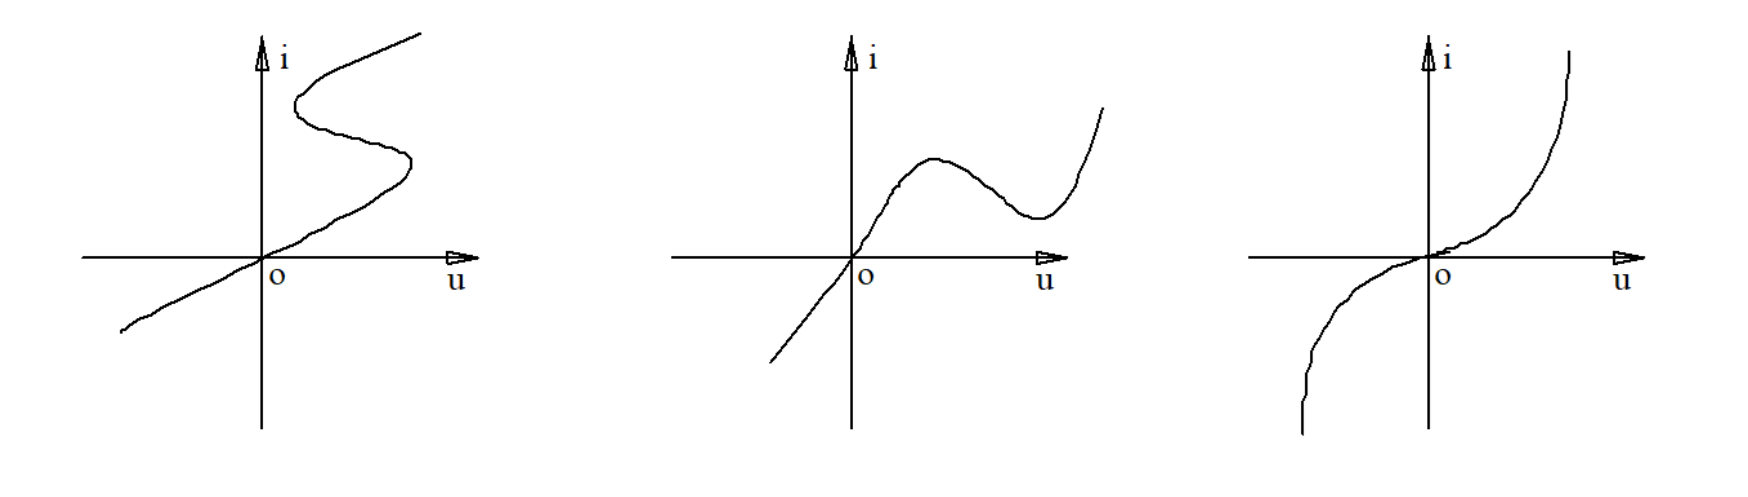
\includegraphics[width=0.6\textwidth]{非线性仪器.png}
			\caption{非线性电阻元件的伏安特性}
		%	\label{fig:name}
		\end{figure}
		\item 常见非线性电阻元件有:电流控制型电阻、电压控制型电阻、既是电流控制型又是电压控制型电阻
		\item 电源可以分为独立源和受控源两种。受控源可以分为四种:压控电压源、流控电压源、压控电流源、流控电流源。受控源的基本特性有输入特性、输出特性和转移特性。 
		\item 输入特性是指控制端电压与电流之间的关系; 输出特性是指控制量为某一常数时,输出端电压与电流之间的关系; 转移特性是指输出量与控制量之间的关系。
		\item 四种理想受控源的转移特性表示如下:\\
		1)VCVS:$\mu$=u1/u2,称之为转移电压比;\\
		2)CCVS:$\gamma$=u2/i1,称之为转移电阻;\\
		3)VCCS: $\mathrm{g}$=i2/u1,称之为转移电导;\\
		4)CCCS:$\beta$=i2/i1,称之为转移电流比。
		
	\end{enumerate}
	% ---
	
	
	
	% 实验前思考题
	\subsection{实验预习题}
	
	% 思考题1
	\begin{question}
		预习了解电路基本元件及其伏安特性。\\原理概述部分
	\end{question}
	
	% 思考题2
	\begin{question}
		考虑发热对电阻伏安特性的影响;\\
		电阻发热会导致电阻的分子无规则热运动加剧,对电子运动的阻抗增加,阻值会升高。
	\end{question}
	
	% 思考题3
	\begin{question}
		万用表电压档与电流档的内阻范围以及内阻对测量的影响;\\
		在电压档,内阻的分流会降低电压。所以内阻越高,分流越小,测量误差越小;\\
		在电流档,内阻的压降会使实际电流减小。所以内阻越小,压降越小,测量误差越小。
	\end{question}
	\begin{question}
		受控源和独立源相比有何异同点?比较两种受控源的代号、控制量与被控制量的关系如何?\\
		独立源的输出电流或电压保持恒定不变,受控源的输出电流或电压可通过改变控制端来改变。\\
		CCVS,控制量为输入电流,被控制量为输出电压;\\
		 VCCS,控制量为输入电压,被控制量为输出电流。
		 \end{question}
		 \begin{figure}[htbp]
		 	\centering
		 	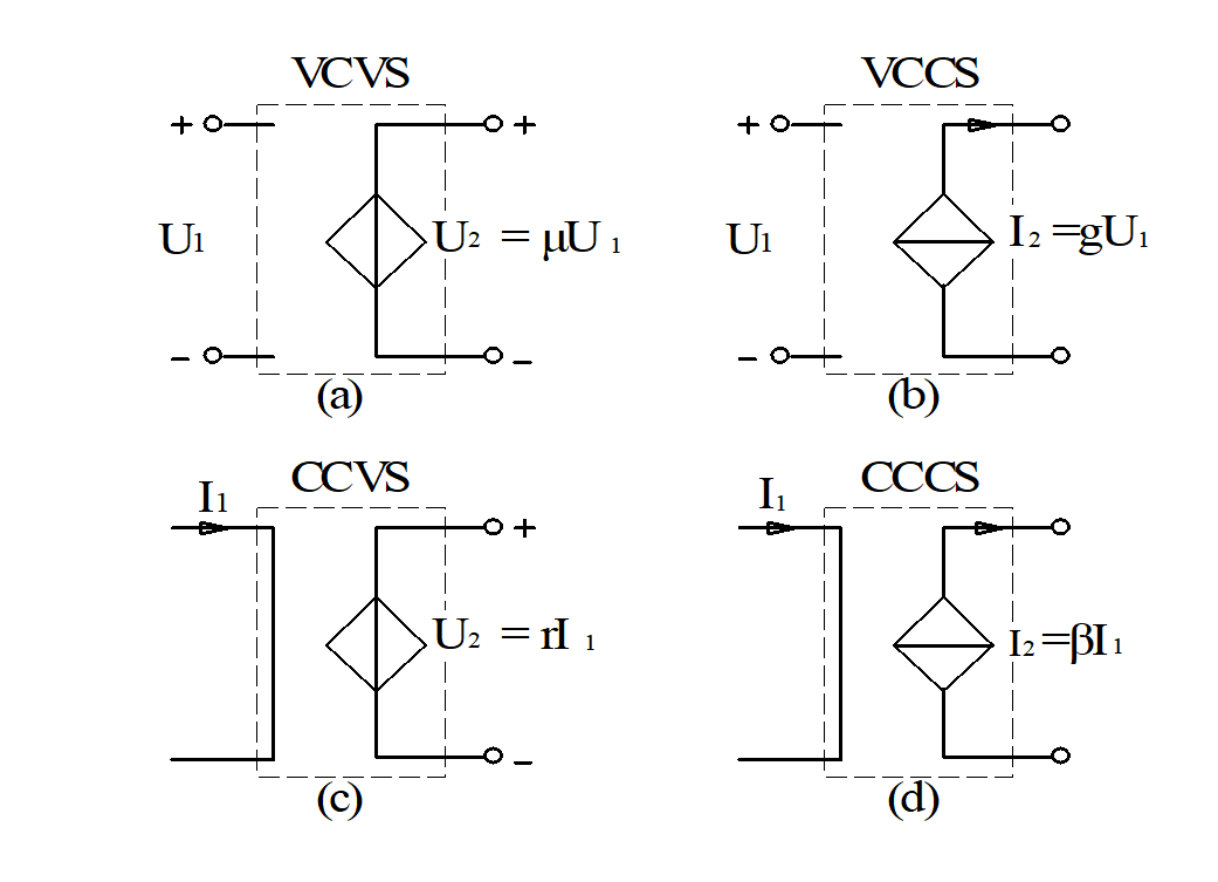
\includegraphics[width=0.5\textwidth]{四种.png}
		 	\caption{四种受控源}
		 %	\label{fig:name}
		 \end{figure}
	
	\begin{question}
		两种受控源中的g、$\gamma$的意义是什么?如何测得?\\
		g为流控电压源的转移电阻,是输出电流与输入电压之比。\\
		$\gamma$为压控电流源的转移电导,是输出电流与输入电压之比。
	\end{question}
	\begin{question}
		受控源输入输出是否符合能量守恒,其中的能量转移是怎么进行的?\\
		受控源输入输出符合能量守恒;受控源的输出能量来自于电路的其他部分或外部提供,而不是受控源本身。
	\end{question}
	% 实验记录	
	\clearpage
	
	% 顶栏
	\begin{table}
		\renewcommand\arraystretch{1.7}
		\centering
		\begin{tabularx}{\textwidth}{|X|X|X|X|}
			\hline
			专业: & 物理学 & 年级: & 2022级 \\
			\hline
			姓名: & 黄罗琳、王显 & 学号: & 22344001、22344002\\
			\hline
			室温: &  23℃& 实验地点: & A522 \\
			\hline
			学生签名:& 见\textbf{附件}部分 & 评分: &\\
			\hline
			实验时间:& 2024/3/6 & 教师签名:&\\
			\hline
		\end{tabularx}
	\end{table}
	% ---
	

	\section{基本电路元件伏安特性的测量 \quad\heiti 实验记录}
	
	% 实验过程记录
	\subsection{实验内容、步骤与结果}
	\subsubsection{测试线性电阻元件的伏安特性}
	操作步骤记录
	\begin{enumerate}
		\item 用电压表和电流表分别采用方法一(电流表内接法)和方法二(电流表外接法)的两种方法实验。
		\item 通过计算可知当电阻两端功率不超过1W时,最大电压和电流分别为:
		\begin{itemize}
			\item $51\Omega$:$I_{max}=0.14A$,$U_{max}=7.14V$;
			\item $120\Omega$:$I_{max}=0.09A$,$U_{max}=10.95V$;
		\end{itemize}
	根据结果,设定在120$\Omega$实验中的电压不超过8V,51$\Omega$实验中电压不超过6V。
	\item 测量过程均采用0.5V步长进行测量,通过调整电源电压进行注意测量并记录数据。
		\item 完成电流表内接实验后,改变实验电路,进行电流表外接的电路进行实验
		\item 计算电阻值,是根据测量的电压、电流值进行计算,计算结果和拟合图像见实验数据分析。
	\end{enumerate}
	
	
	\begin{figure}[H]
		\begin{minipage}[b]{0.4\linewidth}
		  \centering
		  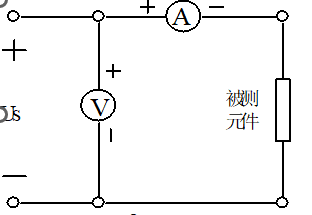
\includegraphics[width=\textwidth]{内接法.png}
		\caption{内接法电路图}
		\end{minipage}
		\hfill
		\begin{minipage}[b]{0.4\linewidth}
		  \centering
		  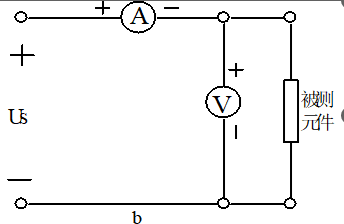
\includegraphics[width=\textwidth]{外接法.png}
	 	\caption{外接法电路图}
		\end{minipage}
		\hfill
	\end{figure}
	
	\begin{figure}[H]
		\begin{minipage}[b]{0.4\linewidth}
		  \centering
		   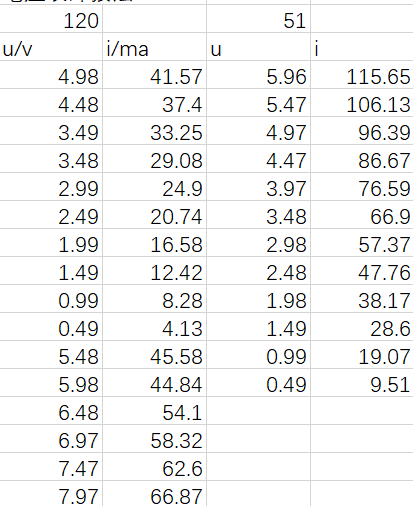
\includegraphics[width=\textwidth]{内接法数据.png}
	 	\caption{内接法实验数据}
		\end{minipage}
		\hfill
		\begin{minipage}[b]{0.4\linewidth}
		  \centering
		  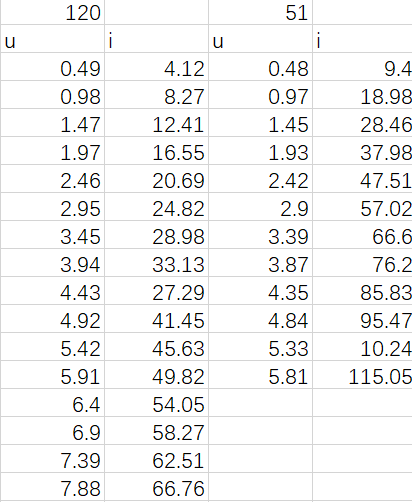
\includegraphics[width=\textwidth]{外接法数据.png}
	 	\caption{外接法实验数据}
		\end{minipage}
		\hfill
	\end{figure}

	
		
	 
	 
	 	
	 
	 
		\subsubsection{测试非线性电阻12V白炽灯的伏安特性}
		\begin{enumerate}
			\item 最大电压不能超过 12V,防止功率过大,烧坏元件。
			\item 电路图如图7所示,根据小灯泡的预估阻值,采取电流表外接的方法进行测量。
		
		\end{enumerate}
	%	\begin{enumerate}
		\begin{figure}[H]
			\centering
			\begin{minipage}[b]{0.4\linewidth}
				\centering
				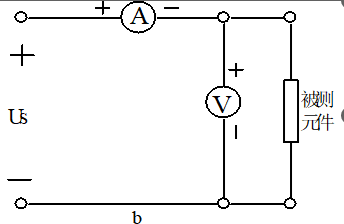
\includegraphics[width=\textwidth]{外接法.png}
				\caption{测量电路图}
				\label{白炽灯测量电路图}
			\end{minipage}
			\hfill
			\begin{minipage}[b]{0.4\linewidth}
				\centering
				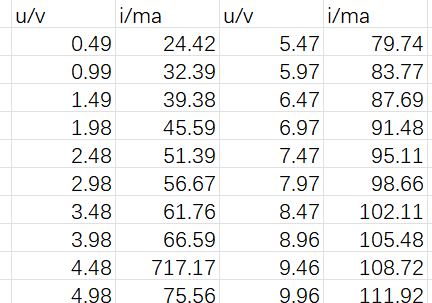
\includegraphics[width=\textwidth]{小灯泡实验数据.png}
				\caption{白炽灯测量实验数据}
				\label{白炽灯测量实验数据}
			\end{minipage}
		\end{figure}
	%	\end{enumerate}
		
			\subsubsection{测试直流稳压电源DP832的CH2的伏安特性}
			\begin{enumerate}
				\item 利用电压表测电阻两端电压,然后除以电阻箱的已知电阻计算电流。
				\item 电路图如图9所示。
				
			\end{enumerate}
			\begin{figure}[H]
				\centering
				\begin{minipage}[b]{0.5\linewidth}
					\centering
					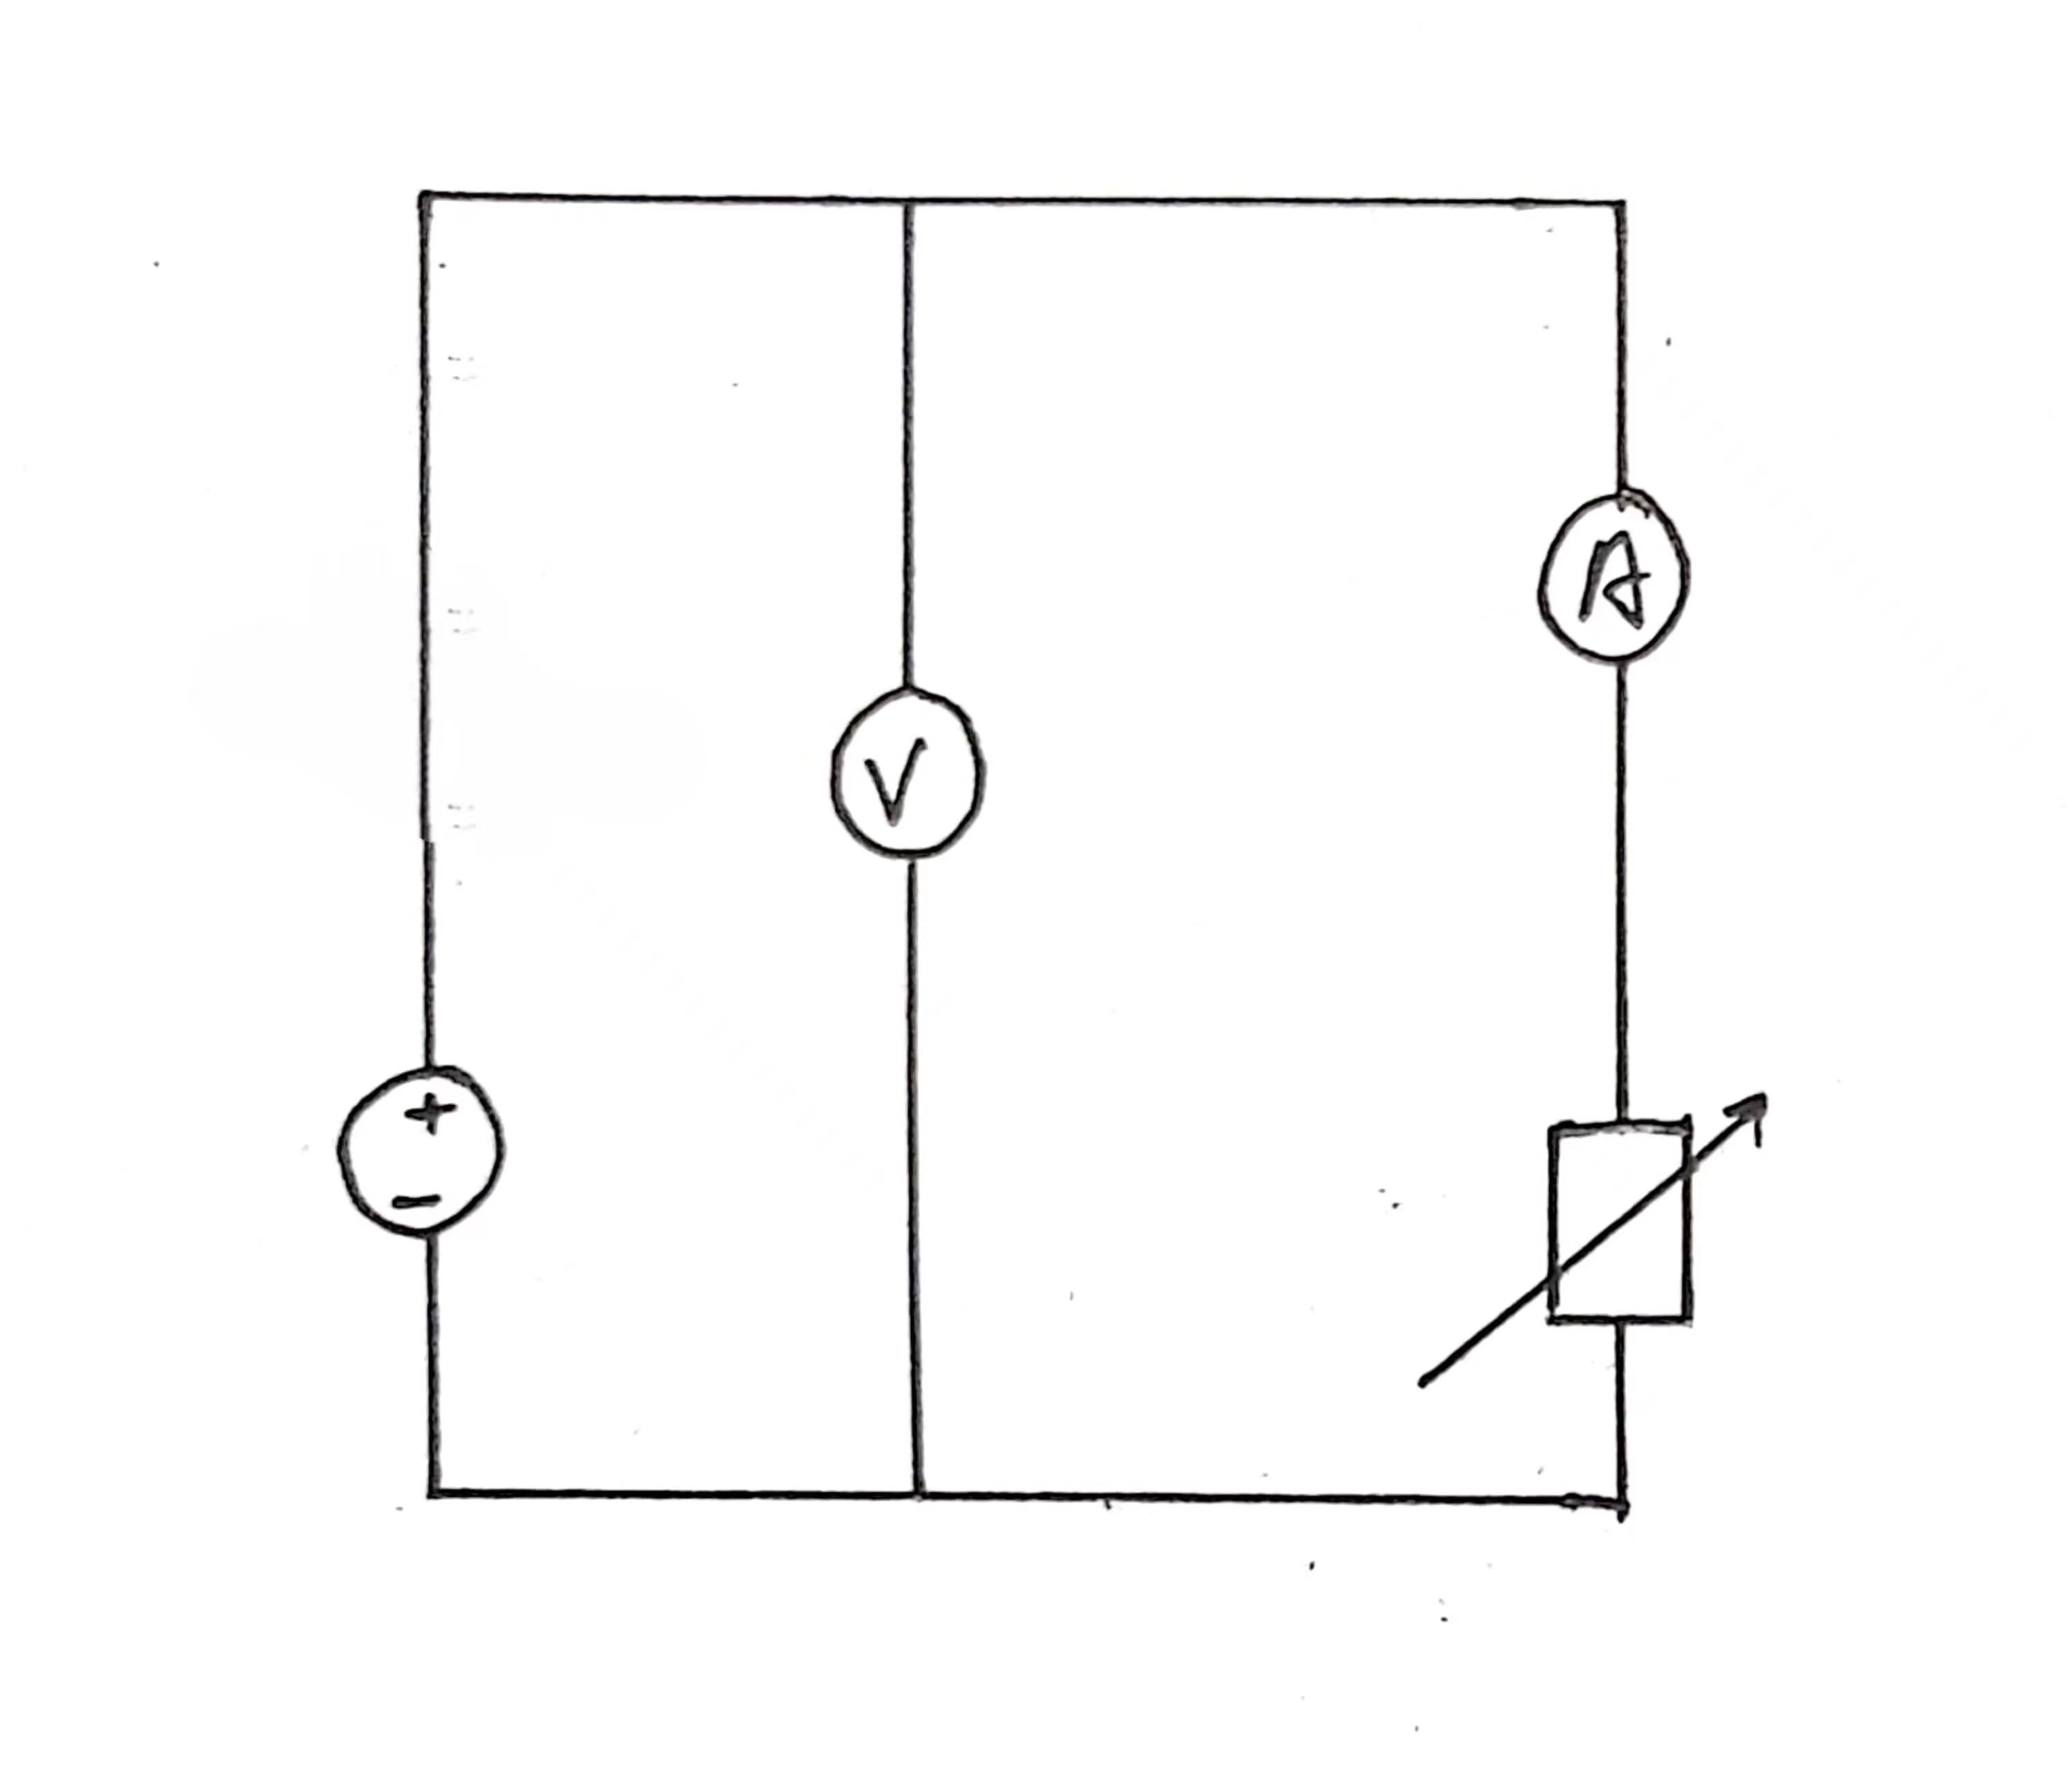
\includegraphics[width=\textwidth]{实验3电路图.jpg}
					\caption{实验电路图}
				\end{minipage}
				\hfill
				\begin{minipage}[b]{0.3\linewidth}
					\centering
					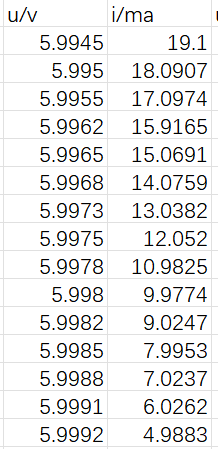
\includegraphics[width=\textwidth]{CH2实验数据.png}
					\caption{CH2实验数据}
					\label{CH2实验数据}
				\end{minipage}
			\end{figure}
		
				\subsubsection{测试数控恒流源(DCS-01)的伏安特性}
			%	\begin{enumerate}
				\begin{figure}[H]
					\centering
					\begin{minipage}[b]{0.5\linewidth}
						\centering
						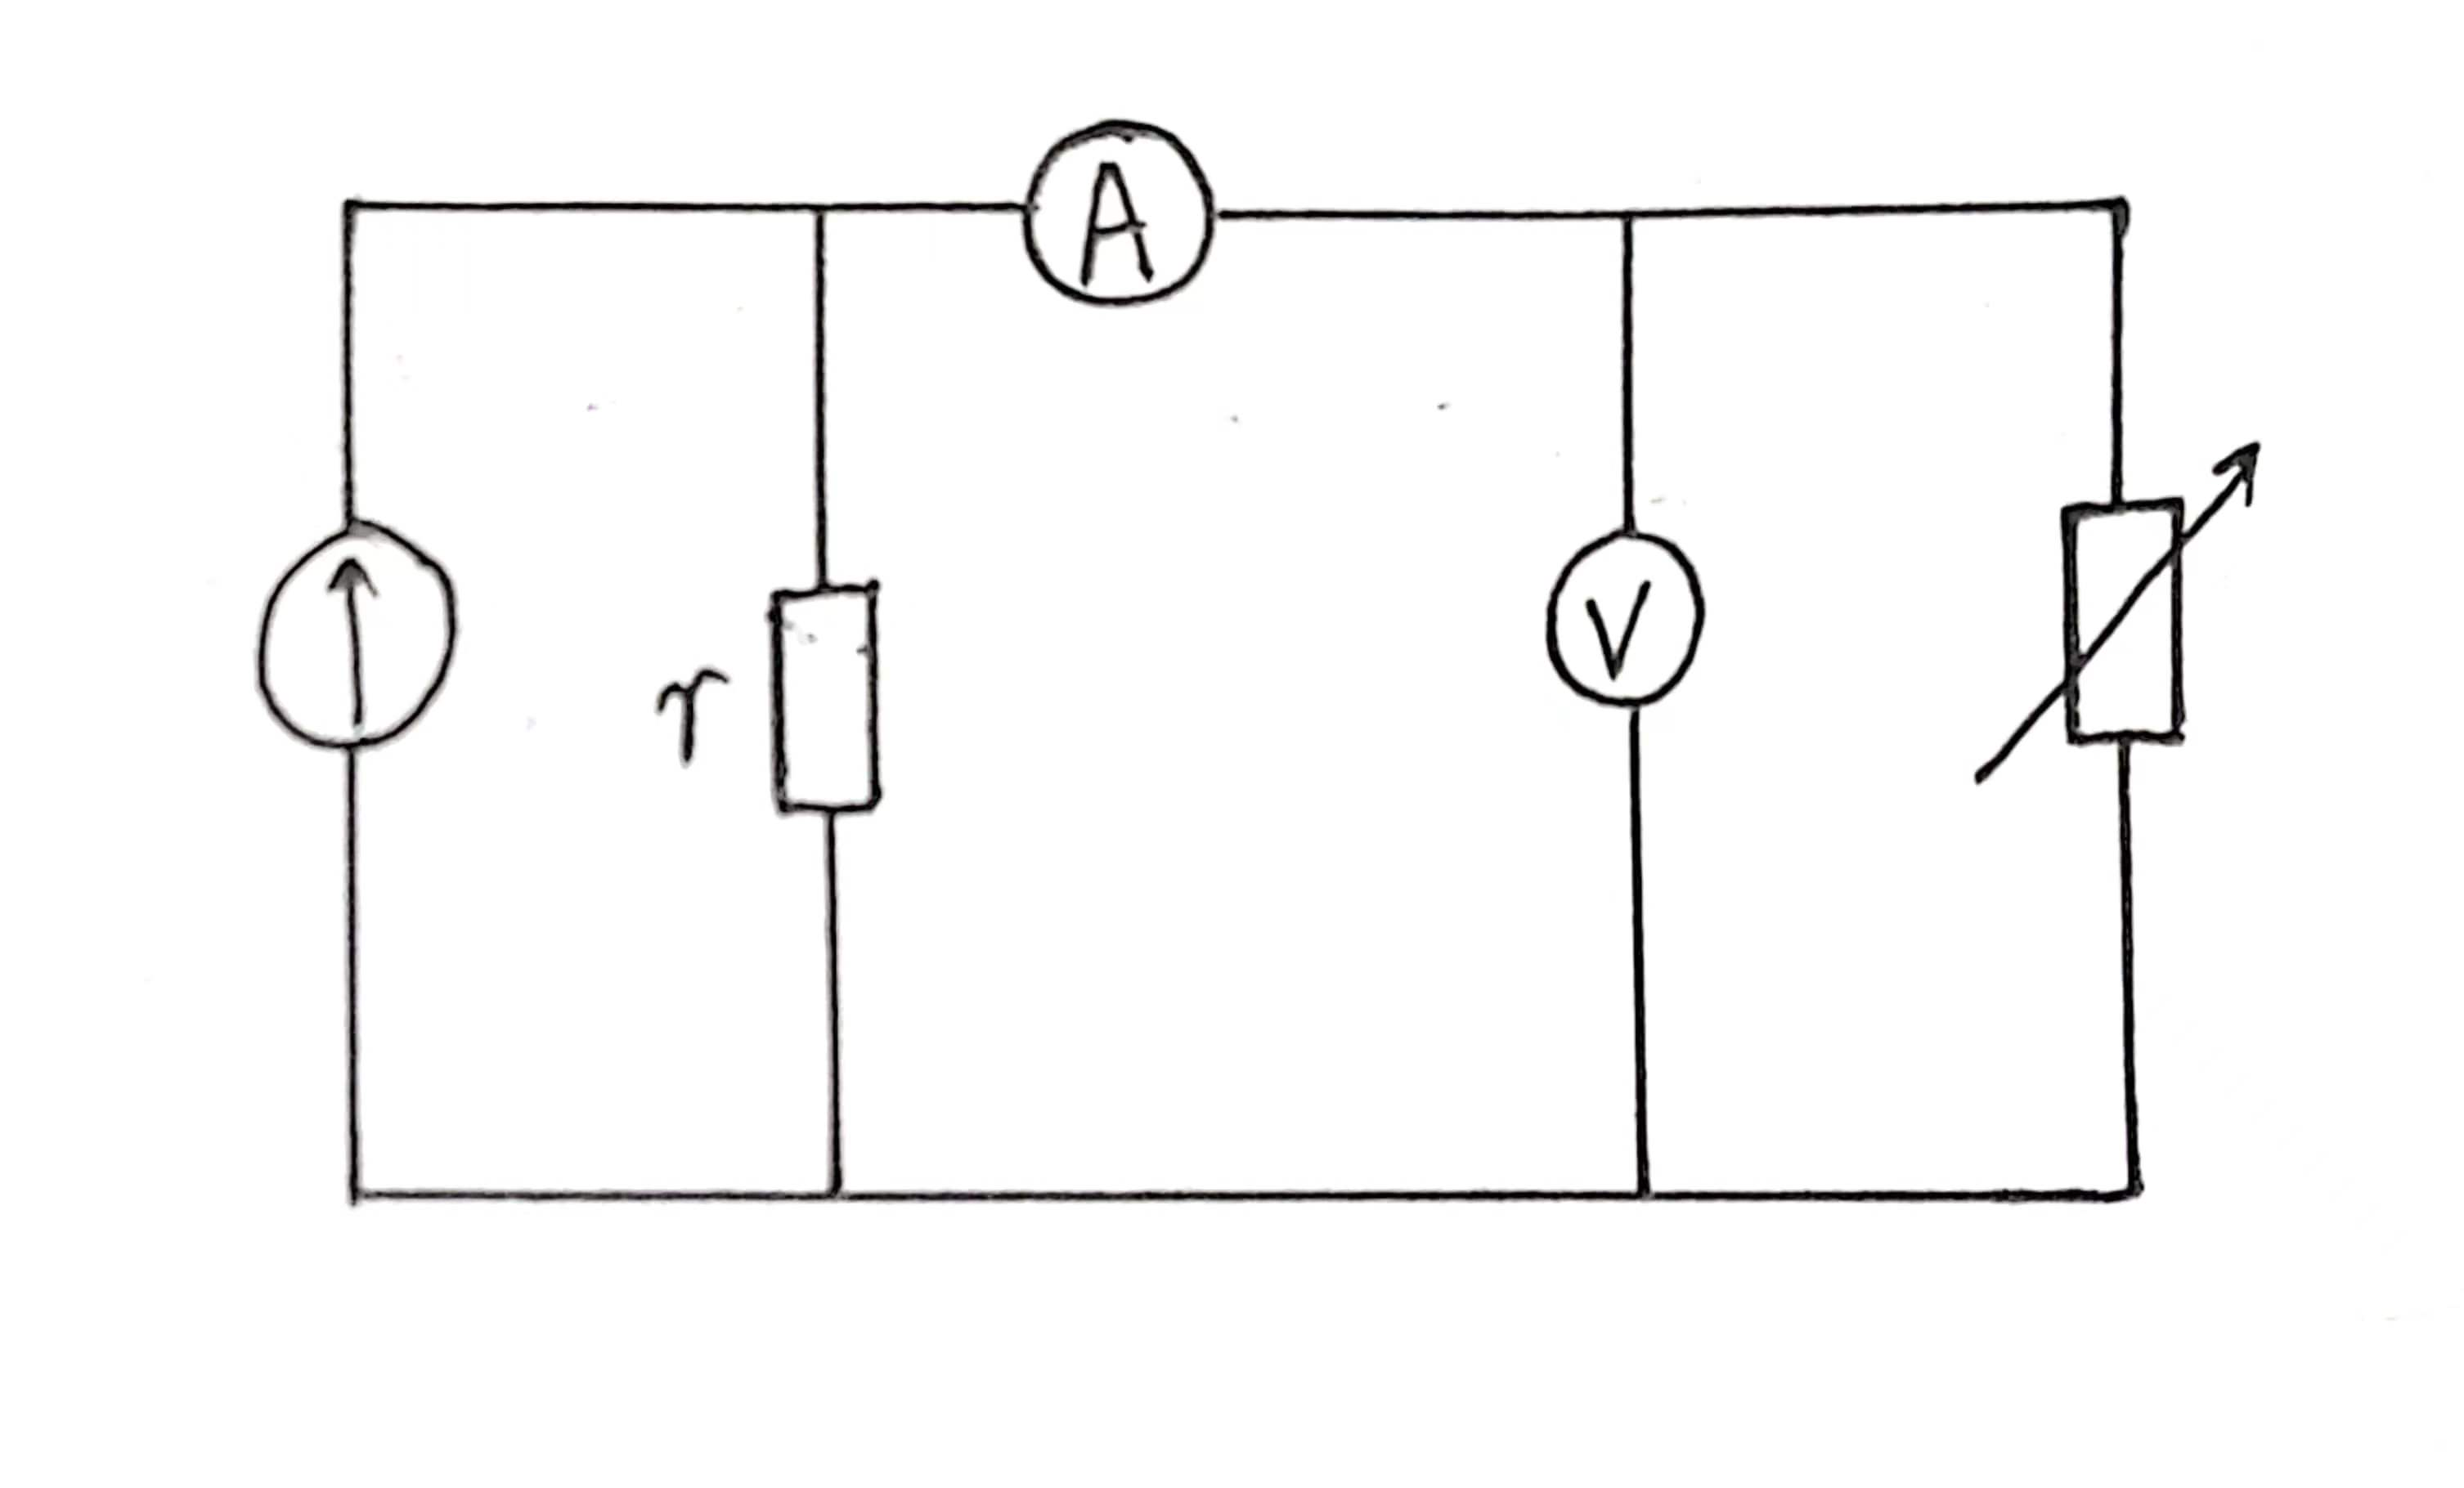
\includegraphics[width=\textwidth]{恒流源.jpg}
						\caption{实验电路图}
						\label{内接法电路图}
					\end{minipage}
					\hfill
					\begin{minipage}[b]{0.4\linewidth}
						\centering
						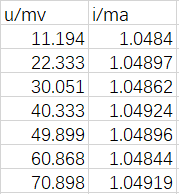
\includegraphics[width=\textwidth]{dcs实验数据.png}
						\caption{数控恒流源(DCS-01)的伏安特性实验数据}
						\label{dcs实验数据}
					\end{minipage}
				\end{figure}
				
					\subsubsection{电流控制电压源(CCVS)基本特性测试}
				\begin{enumerate}
					
					\item 输出特性
					\begin{enumerate}
						\item 输出特性。使 CCVS 控制电流 \(I_1=100\mu A\),负载电阻分别为 \(1K\Omega\)、\(3K\Omega\)、\(5K\Omega\) 时,用万用表测量输出电压 \(U_2\) 和输出电流 \(I_2\),将数据填入表中。
						\item 转移特性及输入特性。使 CCVS 负载 \(RL = 2K\Omega\),改变控制量 \(I_1\) 大小,用万用表测量控制端电压 \(U_1\) 及输出电压 \(U_2\),记录数据。
					\end{enumerate}
				\begin{table}[htbp]
					\centering
					\begin{tabular}{|l|l|l|}
						\hline
						r/$\Omega $ & u输出/V & i输出/mA  \\ \hline
						1k & 6.085 & 6.085  \\ \hline
						3k & 6.136 & 2.028  \\ \hline
						5k & 6.162 & 1.232  \\ \hline
					\end{tabular}
				\end{table}
				\item 转移特性及输入特性\\
				使CCVS负载$RL=2K\Omega $,改变控制量I1大小
				\begin{table}[htbp]
					\centering
					\begin{tabular}{|l|l|l|l|}
						\hline
						实际 & I1输入/mA & u1/v & u2/v  \\ \hline
						0.129 & 0.1 & 0.787 & 6.448  \\ \hline
						0.241 & 0.2 & 2.442 & 8.984  \\ \hline
						0.349 & 0.3 & 8.094 & 9.019  \\ \hline
						0.276 & 0.25 & 3.917 & 8.915  \\ \hline
						0.202 & 0.15 & 1.76 & 8.857  \\ \hline
						0.168 & 0.13 & 1.194 & 8.09  \\ \hline
						0.093 & 0.05 & 0.414 & 4.665  \\ \hline
					\end{tabular}
				\end{table}
			
         	\end{enumerate}
	
	% ---

	
	% 问题记录
	\subsection{实验过程遇到问题及解决办法}
	\begin{enumerate}
		\item 第一个实验中出现了与理论计算不相符的情况(两种方法一测量值偏大,一测量值偏小)而经过初步计算认定两值均偏小,虽然相对大小正确,经分析,可能由于当时天气为回南天,湿度较大,导致电路连接出现因潮湿而出现传输问题,可能会导致数据出现误差。
		\item 第二个实验中起初由于电压较小,灯泡亮度较低,无法确认是否连接正常,可以选择从高电压进行测量,这样可以确认电路安全,也可以保证电路连接正确。
		\item 第三个实验中,由于内电阻接近于零故建立如图9所示电路电路。
		\item 第五个实验中,电路连接有很多难点,经过与老师讨论和同学互助,正确连接了电路,并帮助多位同学完成了电路连接,其中电路板12V供电起初并没有打开,出现了一组错误数据,其在数据记录原始版中有体现,在更正数据之后,得到了初步符合理论计算的数据。
		\item 实验中很多连接需要充分利用各种借口的连接线,此外由于手持式万用表很容易损坏,出现了要更换保险丝的问题。
	\end{enumerate}
	% ---
	
	
	
	% 分析与讨论	
	\clearpage
	
	% 顶栏
	\begin{table}
		\renewcommand\arraystretch{1.7}
		\begin{tabularx}{\textwidth}{|X|X|X|X|}
			\hline
			专业:& 物理学 &年级:& 2022级\\
			\hline
			姓名: & 黄罗琳、王显 & 学号:& 22344001、22344002\\
			\hline
			日期:& 2024/3/6 & 评分: &\\
			\hline
		\end{tabularx}
	\end{table}
	% ---
	
	% 小标题
	\section{基本电路元件伏安特性的测量\quad\heiti 分析与讨论}
	% ---
	
	% 数据处理
	\subsection{实验数据分析}
	
	%
	\subsubsection{对实验一数据进行线性拟合}
	\begin{enumerate}
		\item 电压表内接法数据拟合
		\begin{figure}[H]
			\centering
			\begin{minipage}[b]{0.4\linewidth}
				\centering
				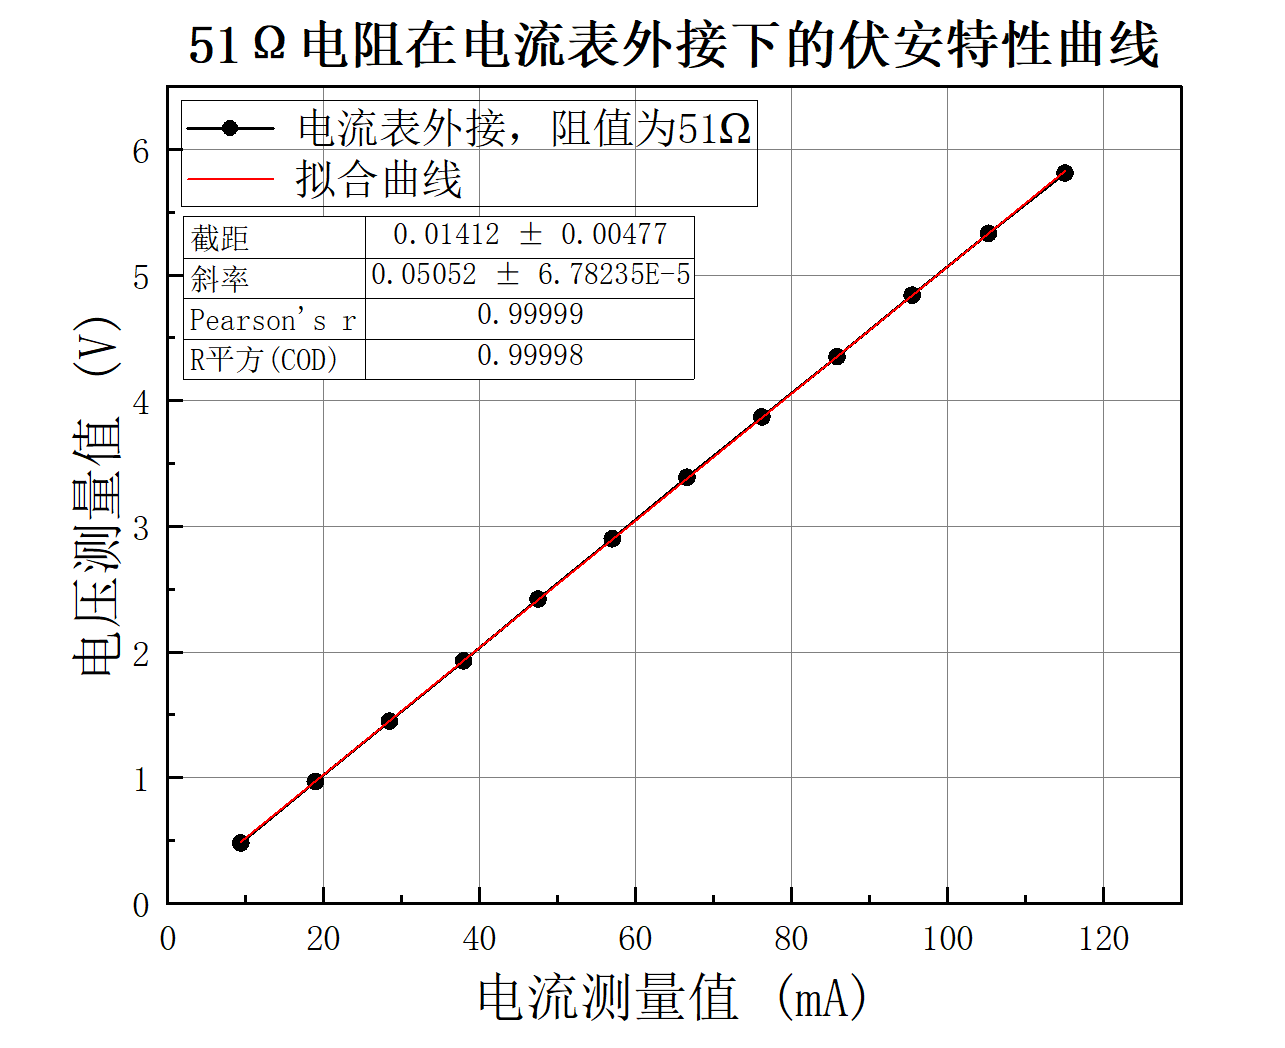
\includegraphics[width=\textwidth]{内接法图片.png}
				\caption{电压表内接51Ω拟合}
				\label{电压表内接51Ω拟合}
			\end{minipage}
			\hfill
			\begin{minipage}[b]{0.4\linewidth}
				\centering
				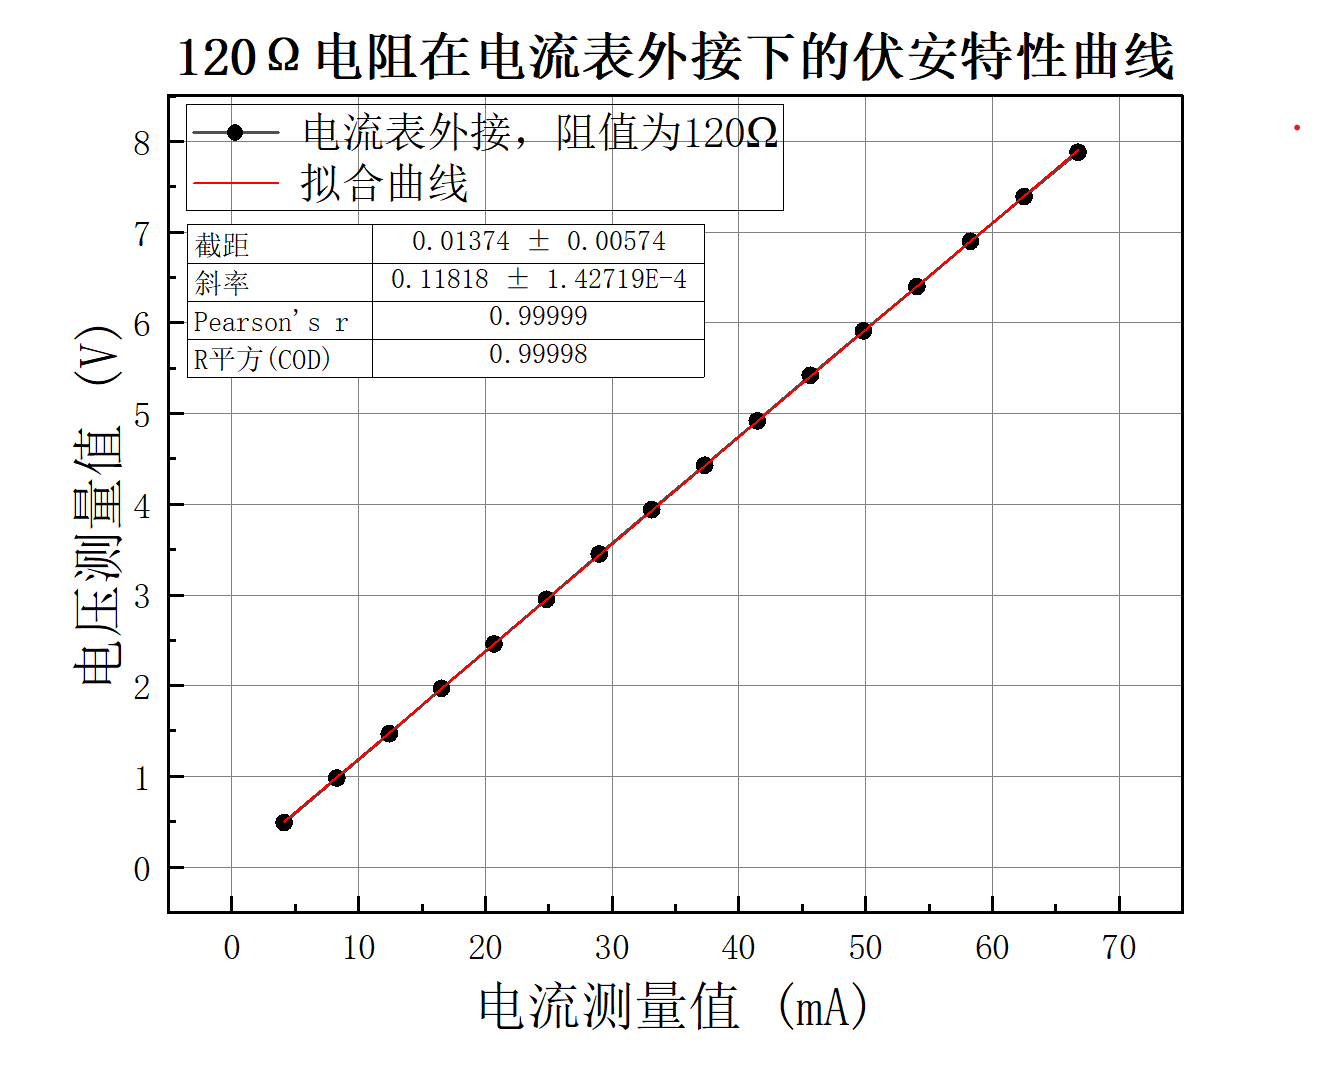
\includegraphics[width=\textwidth]{内接法图片120.png}
				\caption{电压表内接120Ω拟合}
				\label{电压表内接120Ω拟合}
			\end{minipage}
		\end{figure}

			\item 电压表外接法数据拟合
			
			
				\begin{figure}[H]
					\centering
					\begin{minipage}[b]{0.4\linewidth}
						\centering
						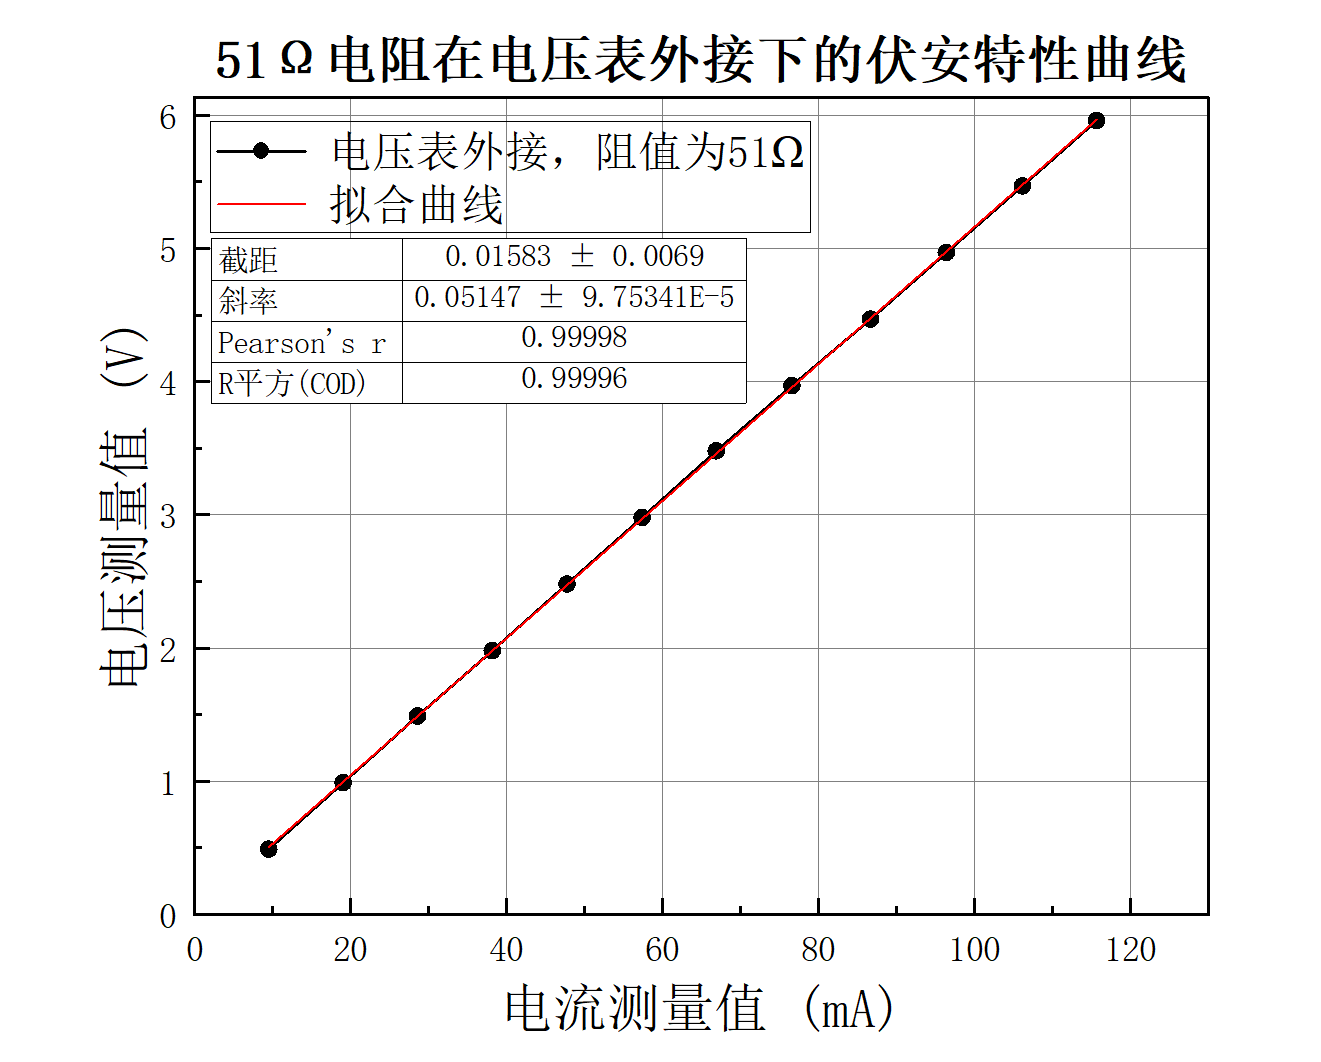
\includegraphics[width=\textwidth]{外接法51.png}
						\caption{电压表外接51Ω拟合}
						\label{电压表外接51Ω拟合}
					\end{minipage}
					\hfill
					\begin{minipage}[b]{0.4\linewidth}
						\centering
						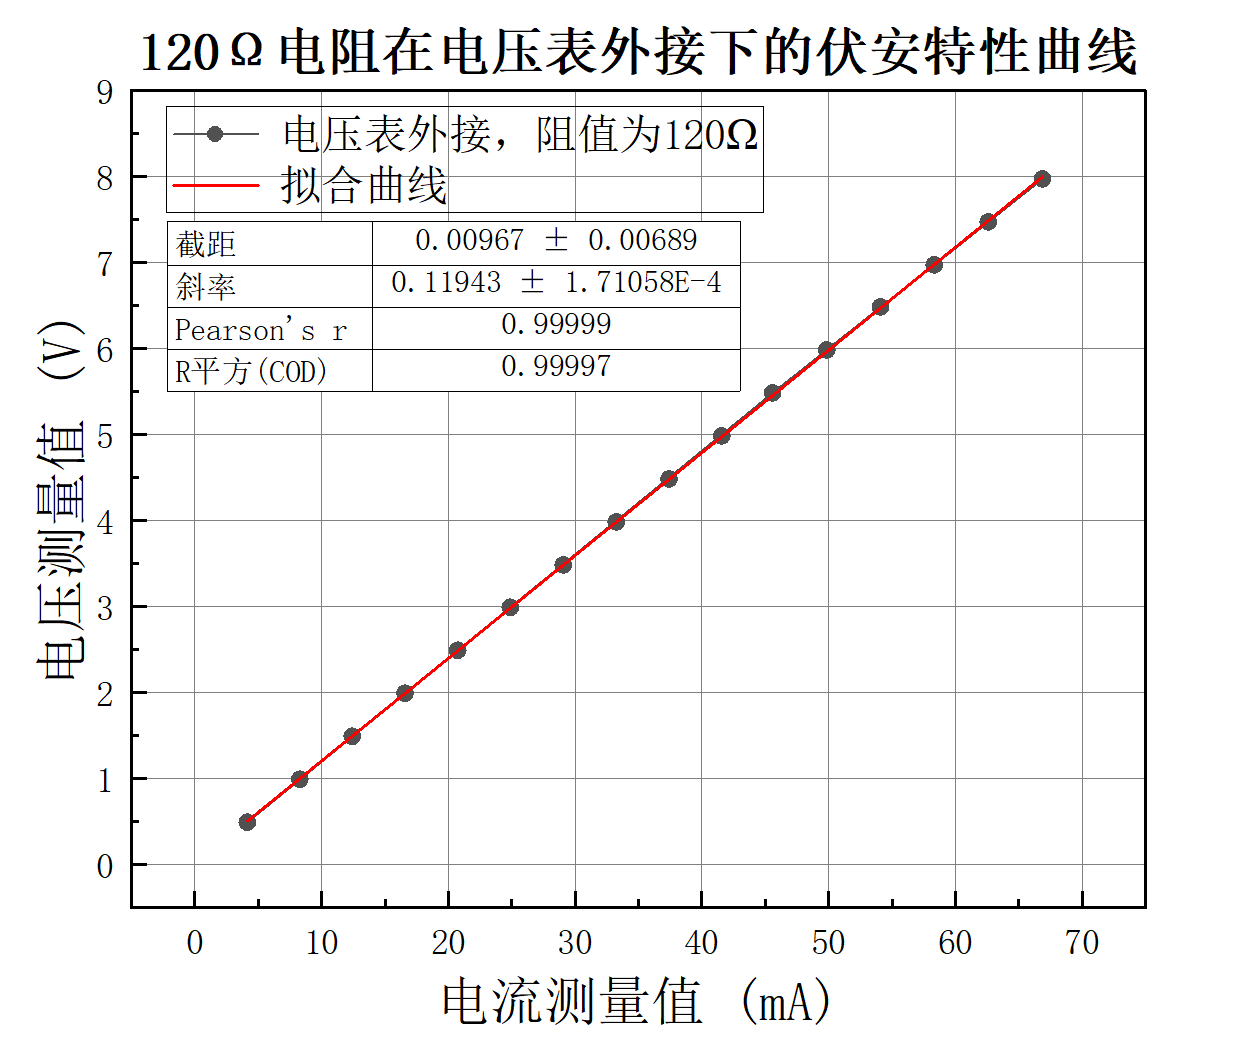
\includegraphics[width=\textwidth]{外接法120.png}
						\caption{电压表外接120Ω拟合}
						\label{电压表外接120Ω拟合}
					\end{minipage}
				\end{figure}
				\item 数据对比
				\begin{figure}[H]
					\centering
					\begin{minipage}[b]{0.45\linewidth}
						\centering
						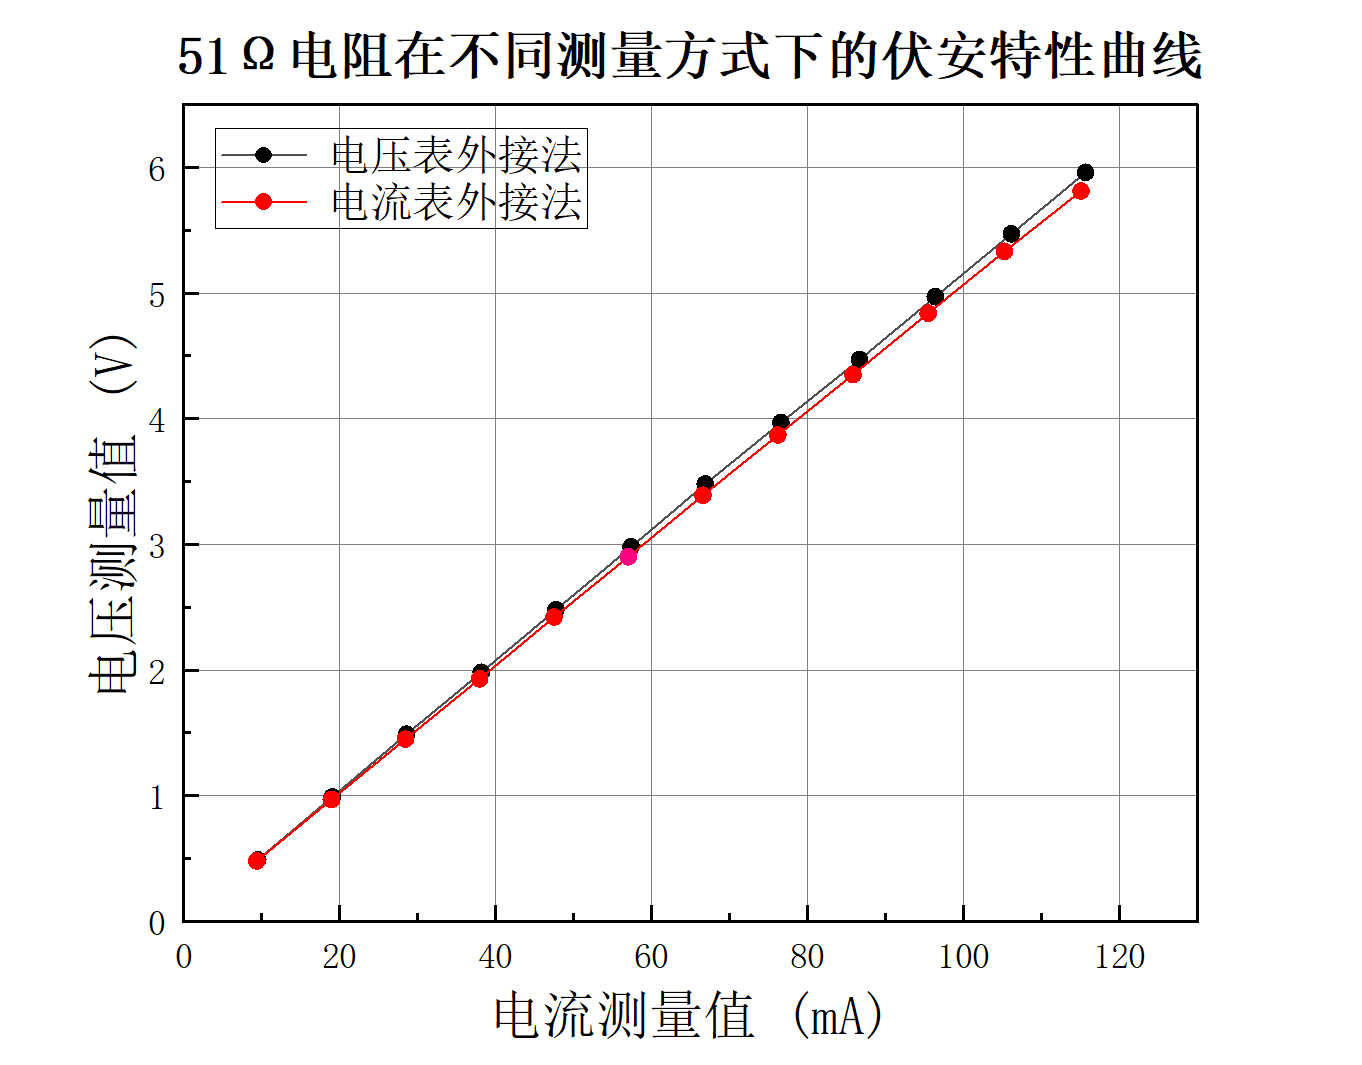
\includegraphics[width=\textwidth]{51数据对比.png}
						\caption{51Ω两种方法数据对比}
						\label{51Ω两种方法数据对比}
					\end{minipage}\hfill
					\begin{minipage}[b]{0.45\linewidth}
						\centering
						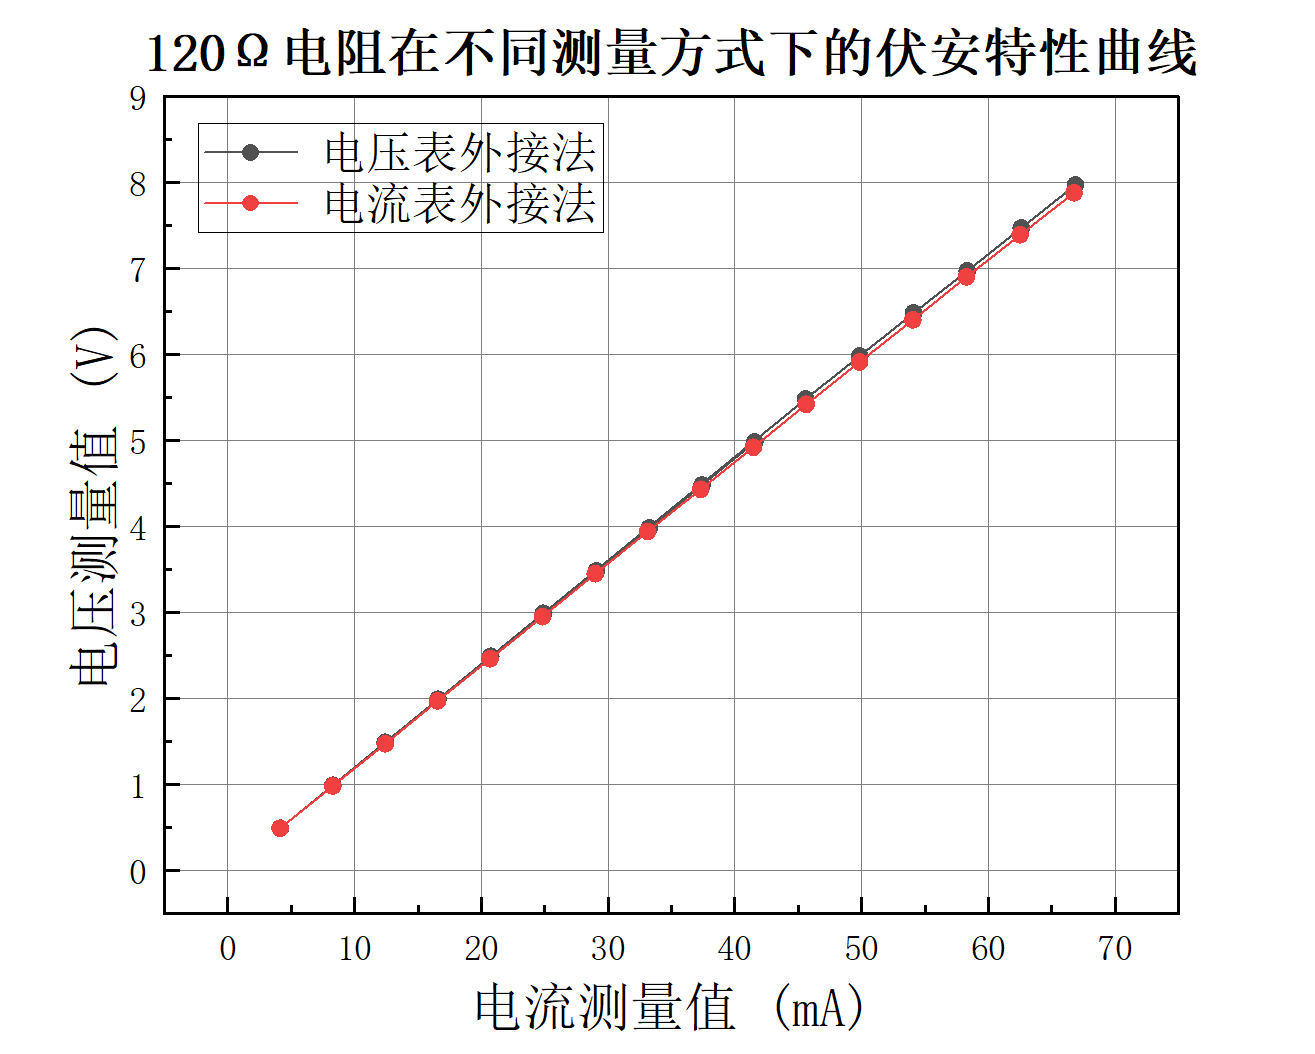
\includegraphics[width=\textwidth]{120数据对比.png}
						\caption{120Ω两种方法数据对比}
						\label{120Ω两种方法数据对比}
					\end{minipage}
				\end{figure}
				\item 数据分析\\
				 内接法结果:$\text{R1=50.52±0. 007}\Omega $
				     \hspace{0.4cm}相对误差:$\text{r1=-0.009}$
				     \hspace{0.4cm}$\text{R2=118.18±0. 02}\Omega$
				     \hspace{0.4cm} 相对误差:$\text{r2=-0.015}$\\
				     外接法结果:$\text{R1=51.47±0. 009}\Omega $
				     \hspace{0.4cm} 相对误差:$\text{r1=0.009}$
				     \hspace{0.4cm}  $\text{R2=119.43±0. 02}\Omega $
				     \hspace{0.4cm}相对误差:$\text{r2=-0.00475}$
					 \indent 数据对比和理论分析可知,测量小电阻时外接法误差更小,测量大电阻时内接法误差更小,之后所有实验电路设计的选择均采用此项原则,例如对于恒压源内阻无限小的情况,采用电压表内接(防止电流表内阻影响测量)\\
					 \indent 误差来源分析:正如前文所说,当时空气湿度较大,故对于120$\Omega$的电阻伏安特性的测量与实际不相符,但是相对大小不变,故可认定实验数据准确,仅存在系统误差。
	\end{enumerate}

	\subsubsection{测试非线性电阻 12V 白炽灯的伏安特性}
	\begin{enumerate}
		\item 将实验数据进行绘图。
			\begin{figure}[H]
			\centering
			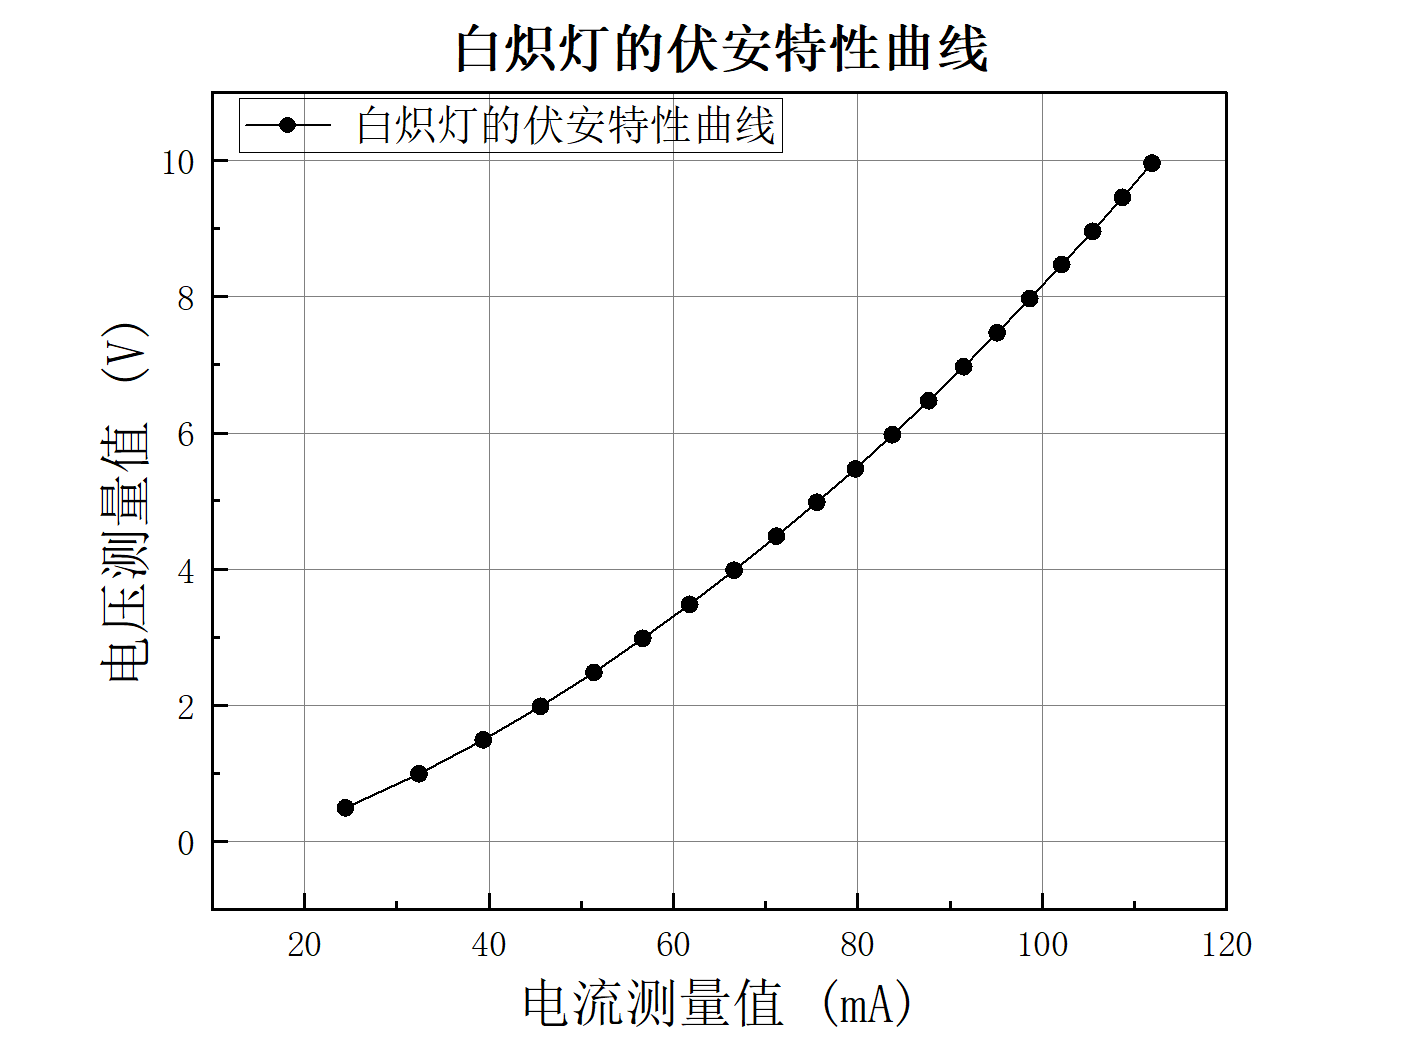
\includegraphics[width=0.4\textwidth]{白炽灯图片.png}
			\caption{白炽灯伏安特性曲线}
			\label{白炽灯伏安特性曲线}
		\end{figure}
		\item 图片数据分析\\
		由图可知,白炽灯(非线性电阻)的伏安特性曲线不是一条直线,电阻值随电压或电流的变化而变化。\\
		\textbf{根据曲线趋势可知,白炽灯的阻值随着电压和电流的增大逐渐升高,其物理意义为:电压电流升高导致灯丝的温度升高,从而加剧了分子的不规则运动,从而影响了金属的导电能力,故会导致阻值升高。}
		
	\end{enumerate}
	
	%
	\subsubsection{测试直流稳压电源(DP831) CH2 的伏安特性}
	\begin{enumerate}
		\item 将实验数据进行绘图。
		\begin{figure}[H]
			\centering
			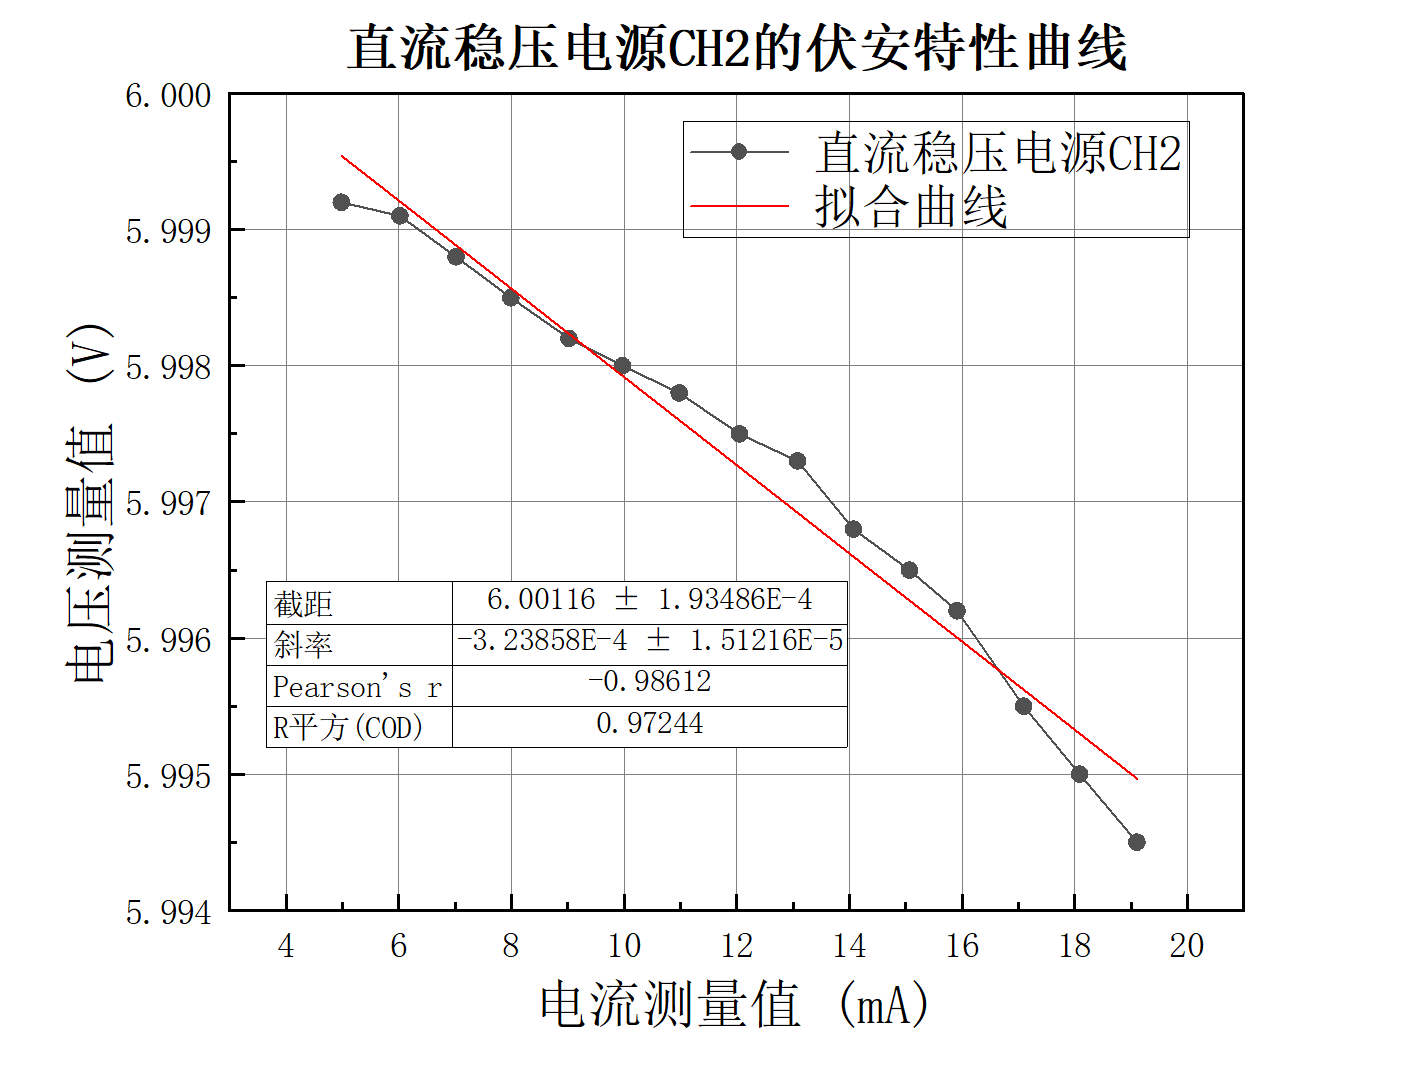
\includegraphics[width=0.4\textwidth]{CH2数据图片.png}
			\caption{直流稳压电源(DP831) CH2 的伏安特性曲线}
			\label{CH2数据图片}
		\end{figure}
		\item 图片数据分析\\
		由图可知,伏安特性曲线不是一条直线,电阻值随电压或电流的变化而变化,这是由于恒压源并非理想电源,存在内阻,故输出电压会产生变化,线性拟合后,斜率的绝对值即为电源内阻。\\
		$r_\text{内}=3.23858\times10^{-4}\Omega.$
		
	\end{enumerate}
		\subsubsection{数控恒流源}
	\begin{enumerate}
		\item 将实验数据进行绘图。
		\begin{figure}[H]
			\centering
			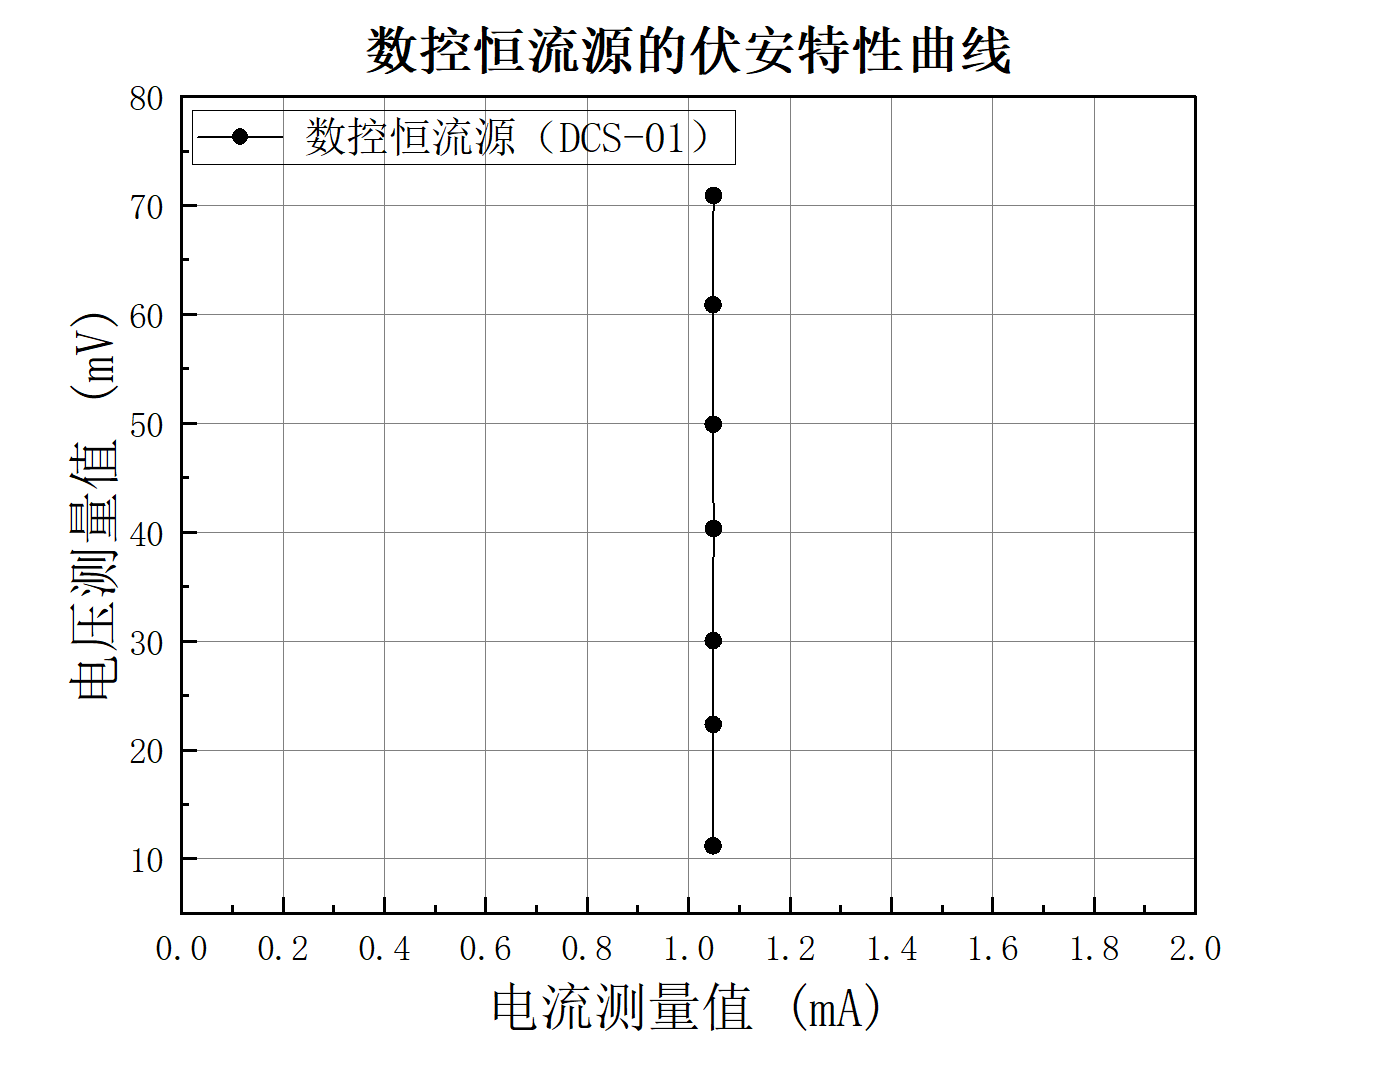
\includegraphics[width=0.4\textwidth]{数控恒流源.png}
			\caption{数控恒流源的伏安特性曲线}
			\label{数控恒流源}
		\end{figure}
		\item 图片数据分析\\
		由图可知,伏安特性曲线近似为一条直线,可以说明恒流源的输出电流恒定,值得一提的是,测量数据发现电流存在极小范围的周期波动,分析其来源可能是由于导线头的不稳定,需要进行手动连接,这可能导致手部颤抖等问题出现接触问题,会导致数据出现波动,但在总体上电流数据恒定,故认定实验成功。
	
	\end{enumerate}
		\subsubsection{电流控制电压源(CCVS)基本特性测试}
	\begin{enumerate}
			\begin{figure}[H]
			\centering
			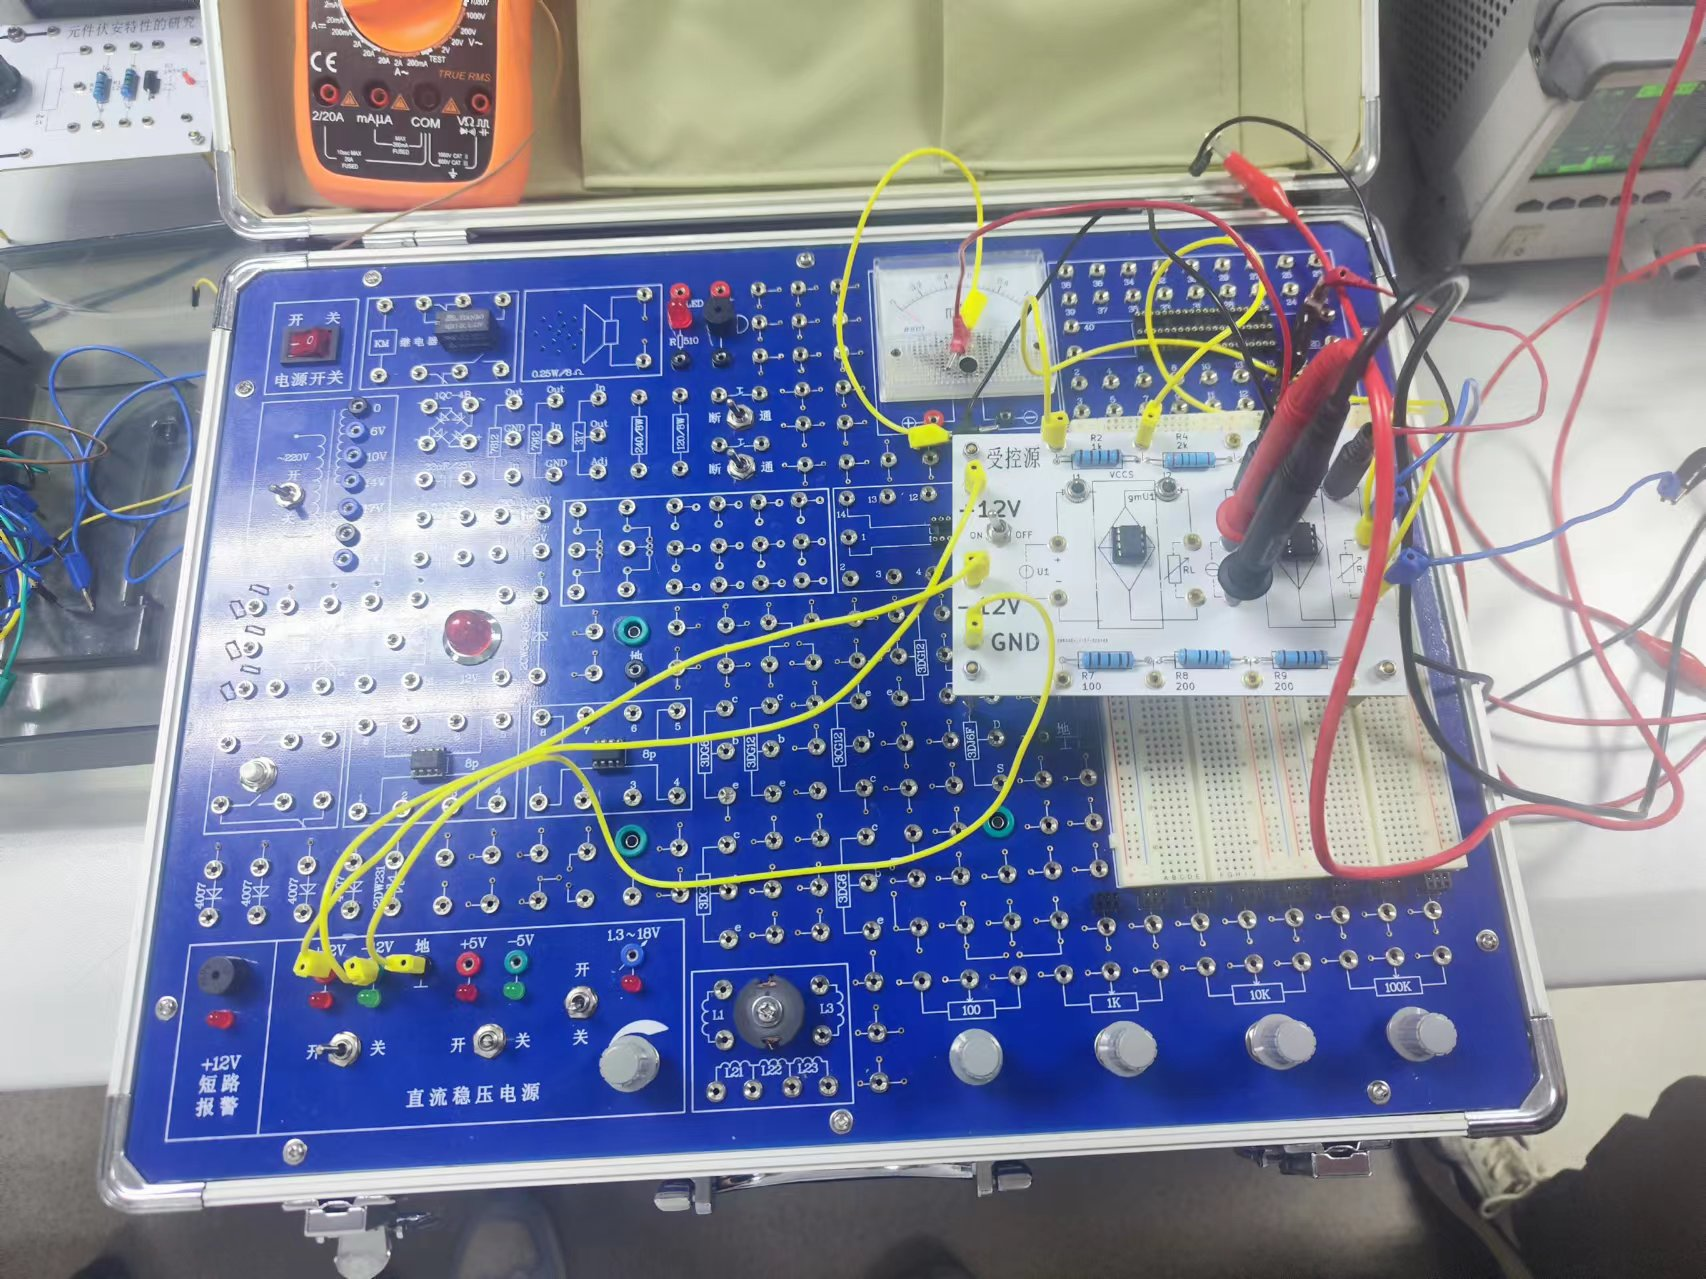
\includegraphics[width=0.3\textwidth]{接线总览.jpg}
			\caption{实验接线总览}
			\label{接线总览}
		\end{figure}
		\item 输出特性
		
		\begin{figure}[H]
			\centering
			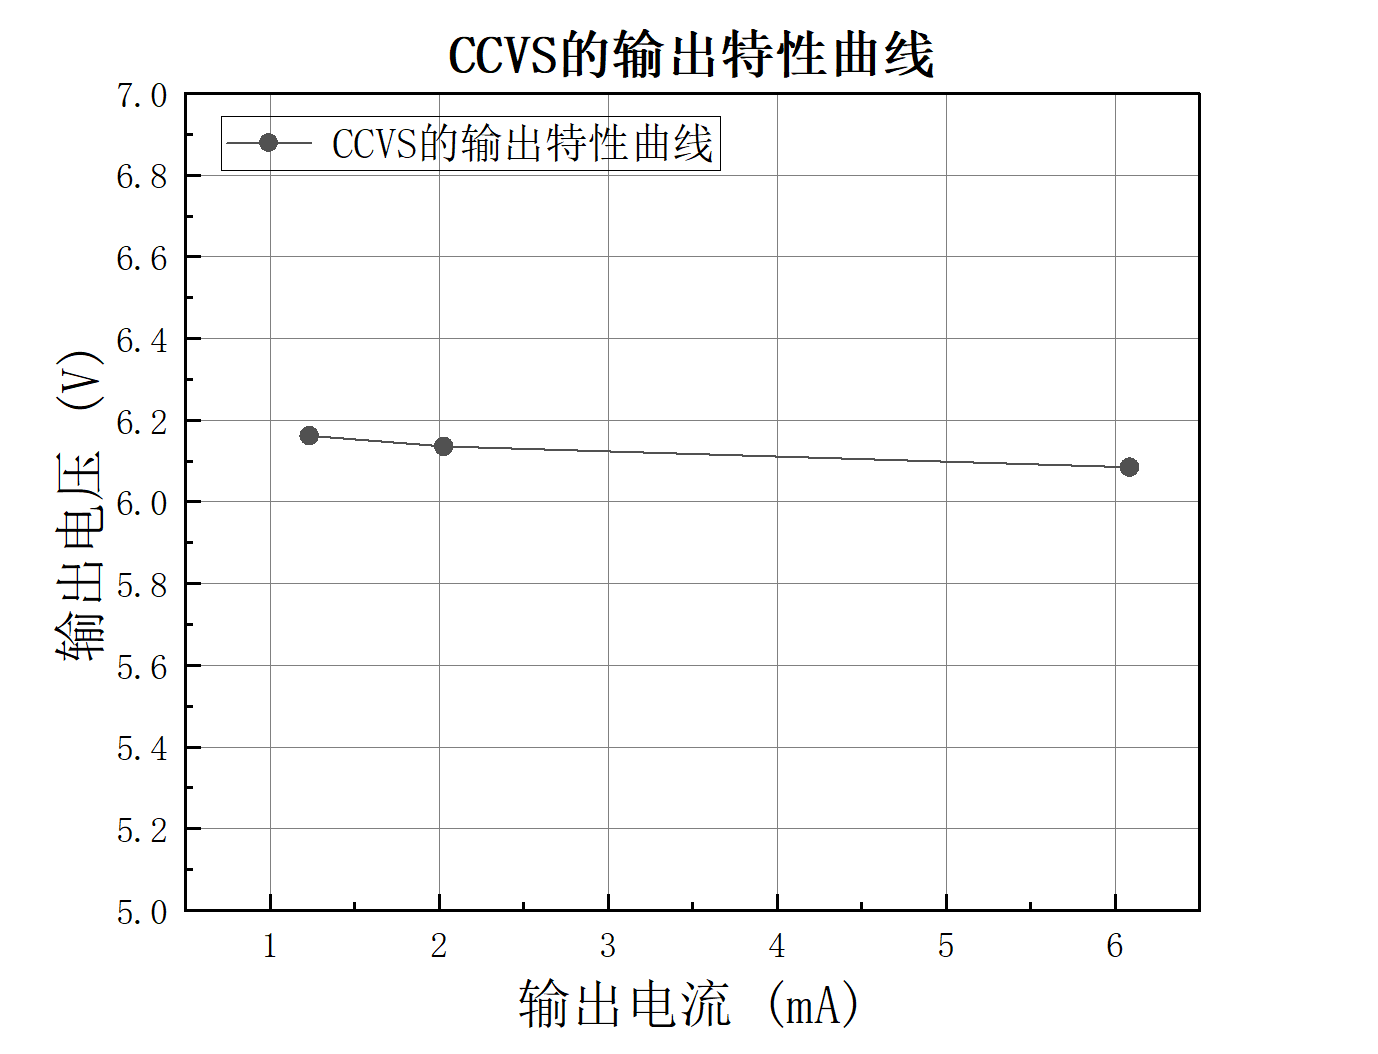
\includegraphics[width=0.4\textwidth]{输出特性.png}
			\caption{电流控制电压源(CCVS)输出特性}
			\label{输出特性}
		\end{figure}
		图片数据分析:由图可知,电流控制电压源,尽管输出电流发生了变化,但是输出电压依旧不变。
		\item 
		
	
	\end{enumerate}

	% 实验后思考题
	\subsection{实验后思考题}
	实验原本思考题在实验前思考题中均完成作答,而本部分为实验后对于之前所写思考题的一个补充
	%思考题1
	\begin{question}
		
	\end{question}
	
	
	
	% 结语部分
	\clearpage
	
	% 小标题
	\section{基本电路元件伏安特性的测量 \quad\heiti 结语}
	% ---
	
	% 总结、杂谈与致谢
	\subsection{实验心得和体会、意见建议}
	\begin{enumerate}
		\item 实验内容较多,基本上需要很繁琐的接线过程,并且需要进行频繁大量的读数,实验数据量和处理过程都很复杂。
		\item 实验仪器要求很高,例如出现了仪器表显和实际测量的数据偏差较大的问题,(例如CCVS过程中我需要去测量实际输入电流,与显示的输入电流相差很大)
		\item 实验仪器手持式万用表存在仪器问题,相对于台式,存在易损坏的问题,建议如果后续实验需要可以加入新的台式万用表,方便实验进行。
	\end{enumerate}
	% ---
	
	
	
	% 附件
	\subsection{附件}
	实验原始数据
	\begin{figure}[H]
		\begin{minipage}[b]{0.3\linewidth}
		  \centering
		  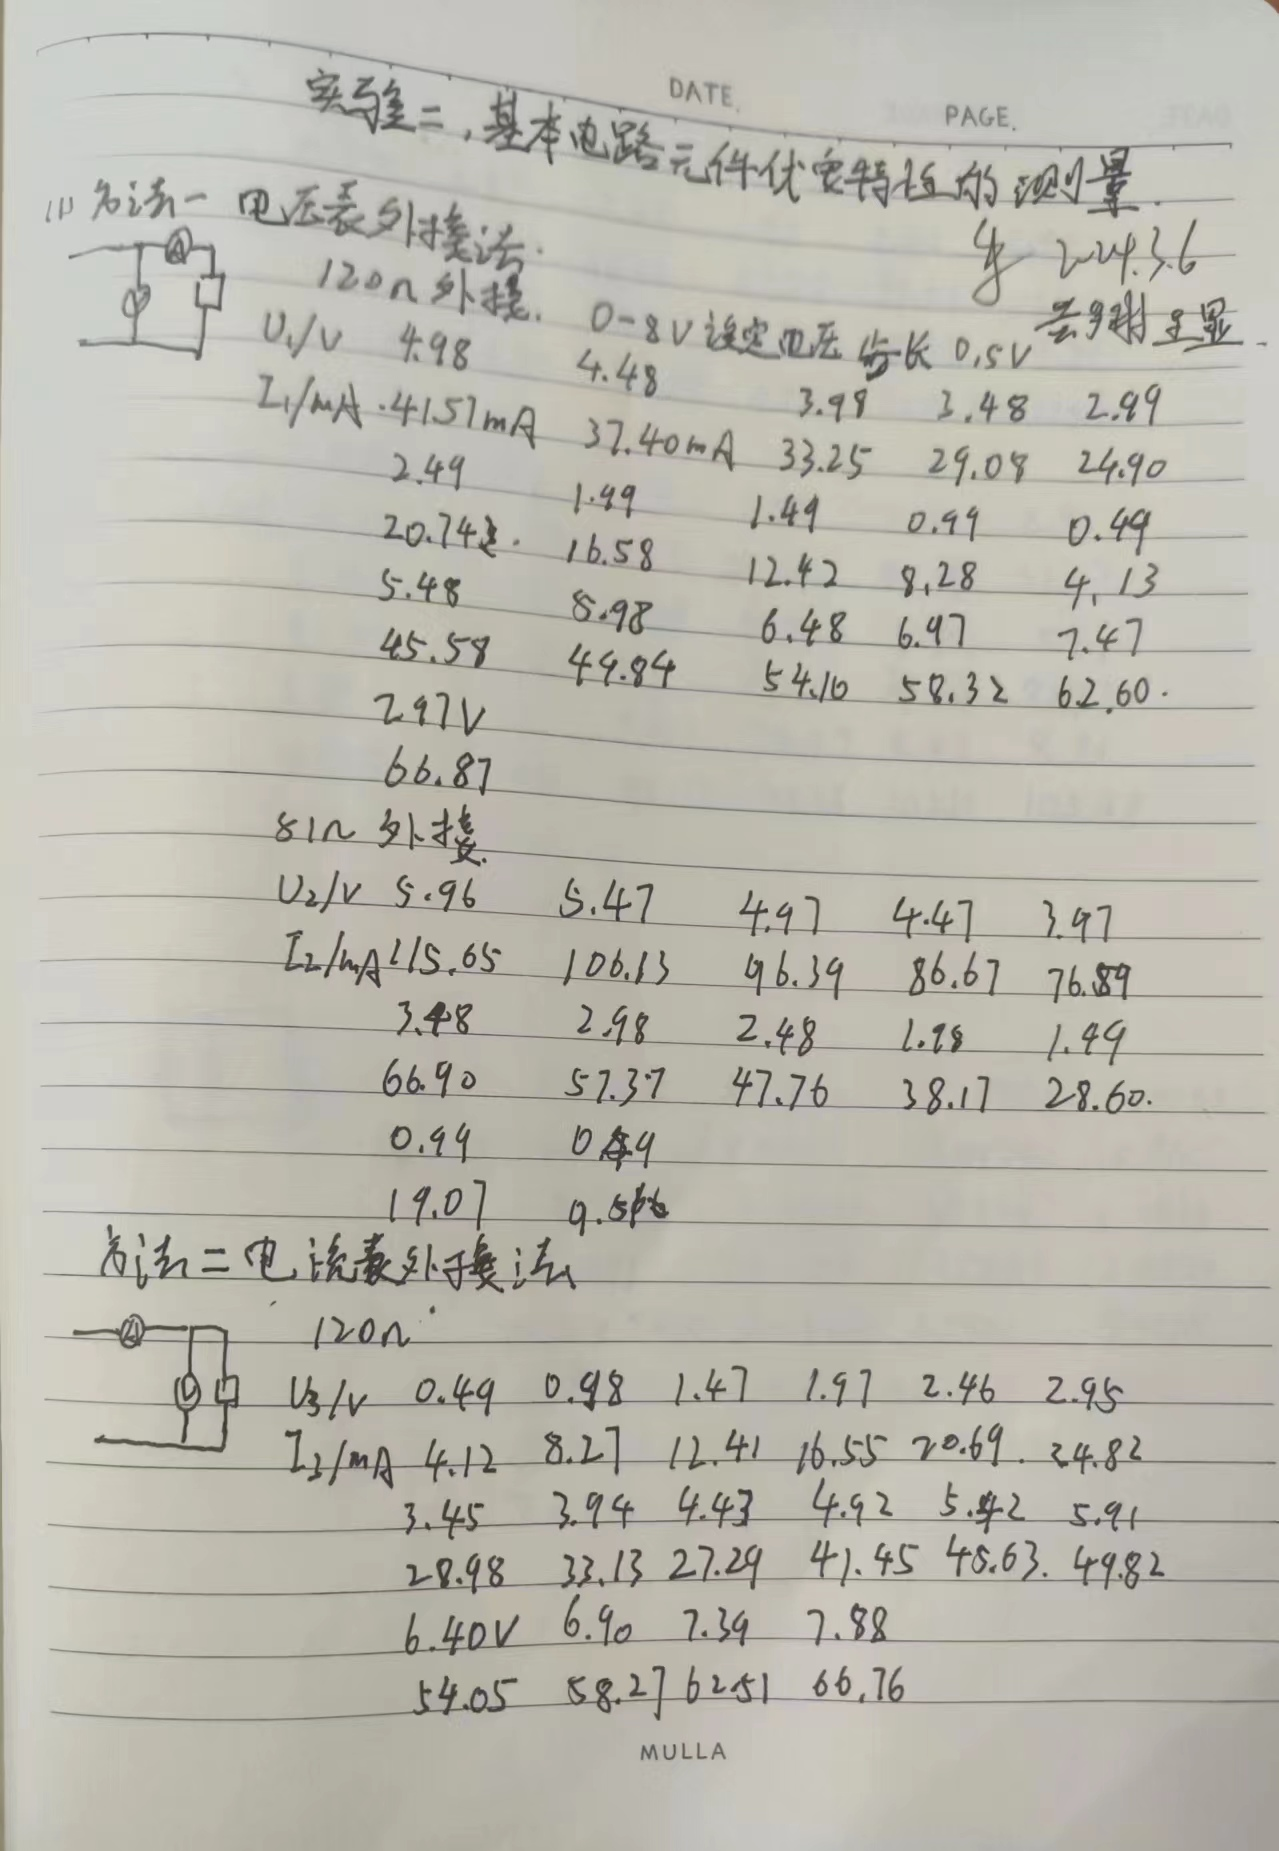
\includegraphics[width=\linewidth]{数据1.jpg}
		  \caption{原始数据1}
		\end{minipage}
		\hfill
		\begin{minipage}[b]{0.3\linewidth}
		  \centering
		  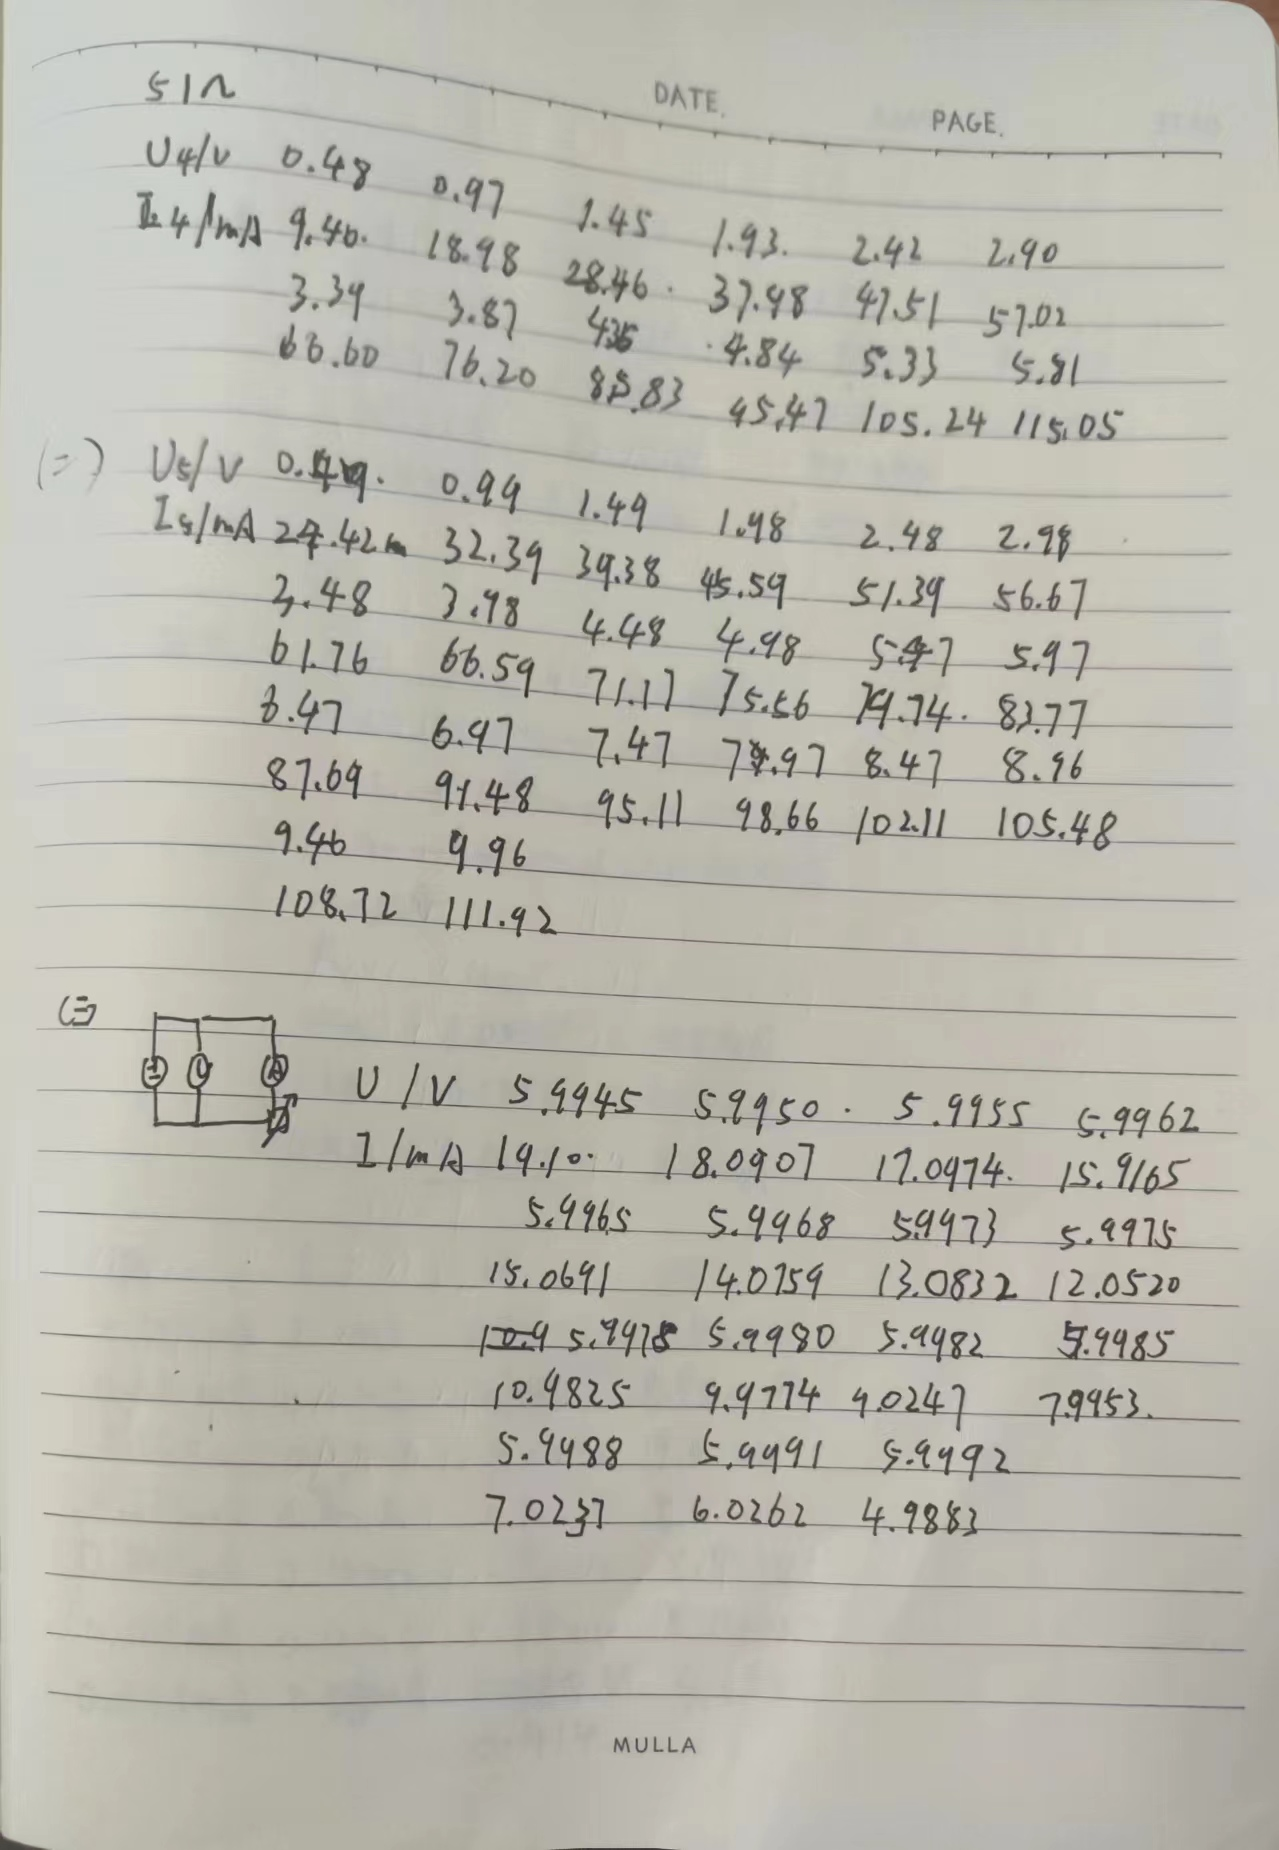
\includegraphics[width=\linewidth]{数据2.jpg}
		  \caption{原始数据2}
		\end{minipage}
		\hfill
		\begin{minipage}[b]{0.3\linewidth}
		  \centering
		  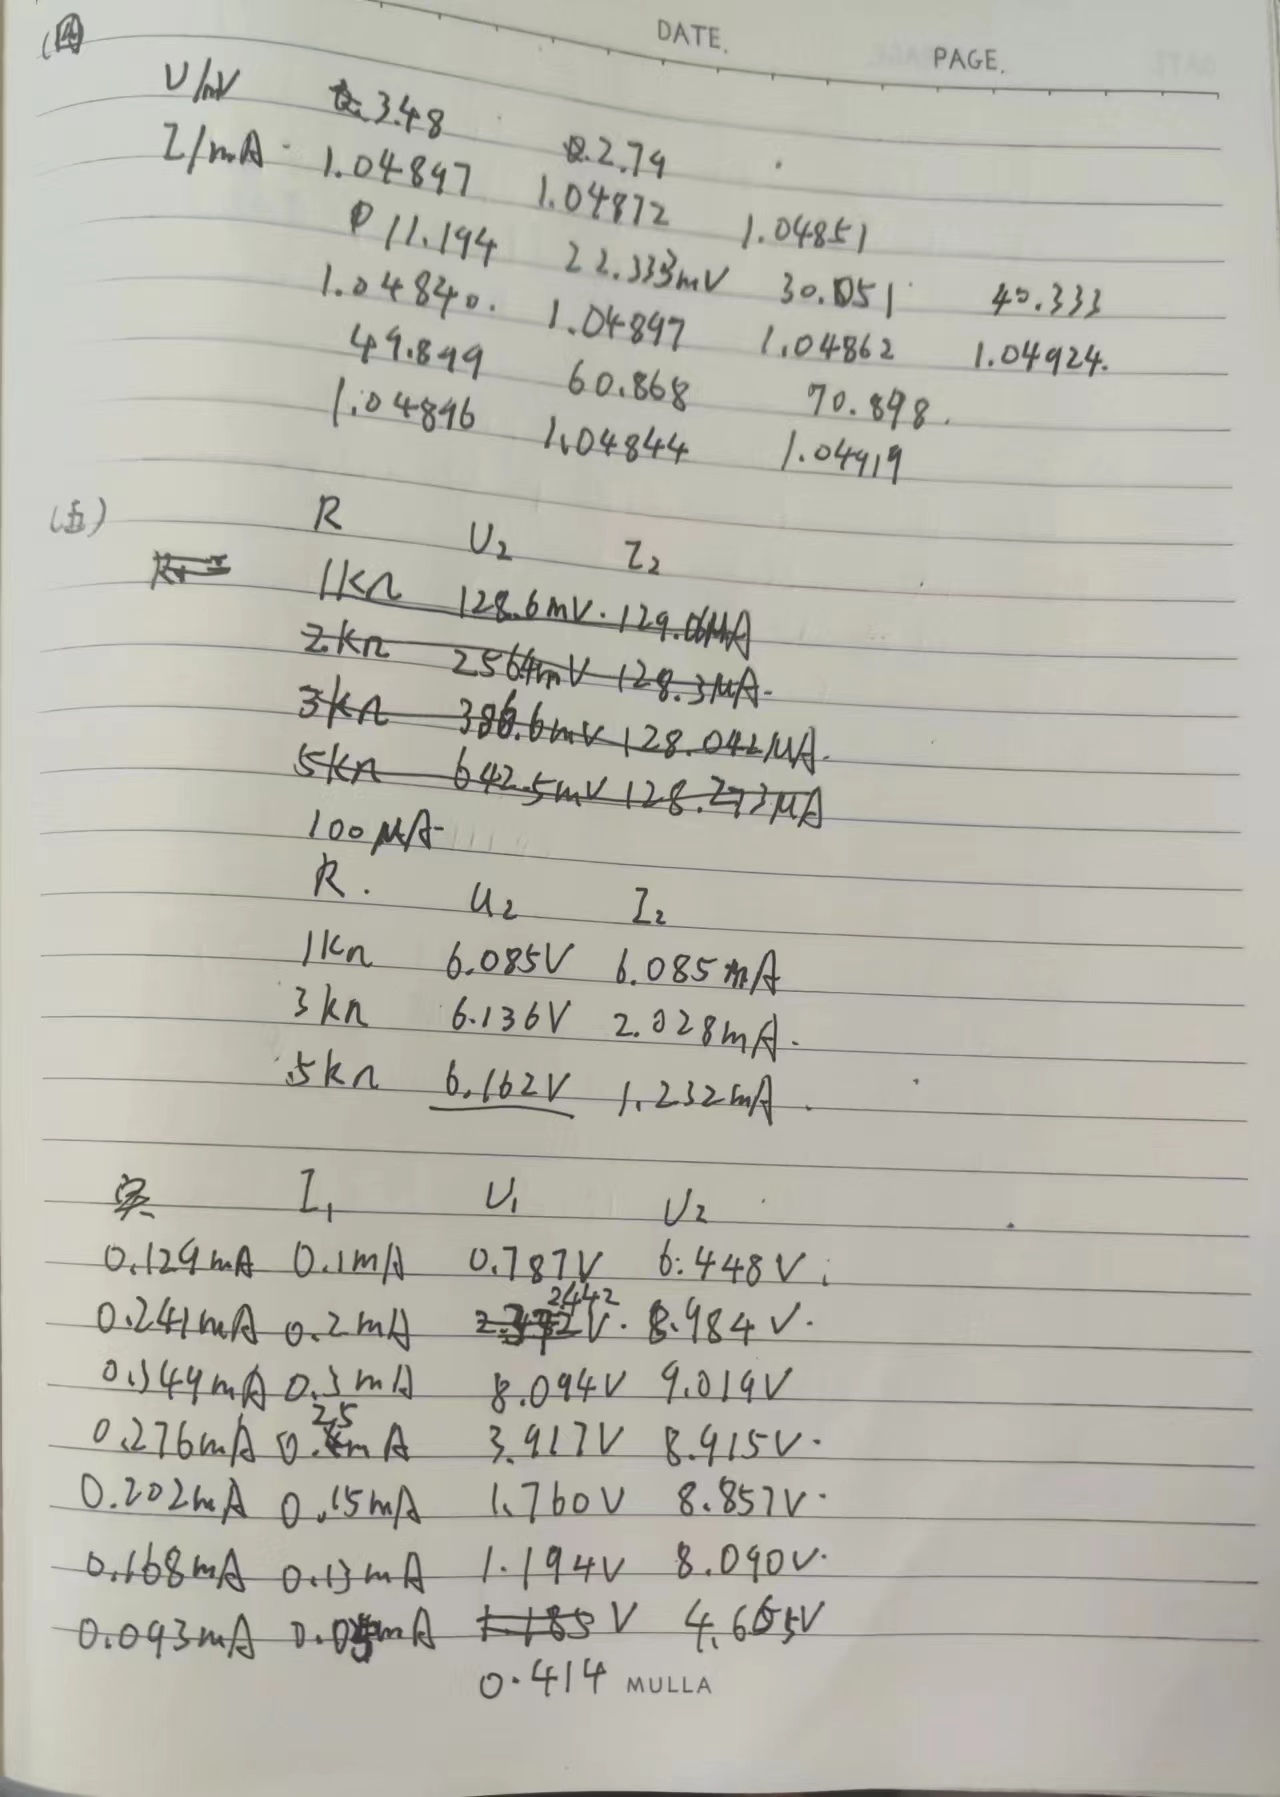
\includegraphics[width=\linewidth]{数据3.jpg}
		  \caption{原始数据3}
		\end{minipage}
	\end{figure}
	试验台桌面整理。
	\begin{figure}[{H}]
		\centering
		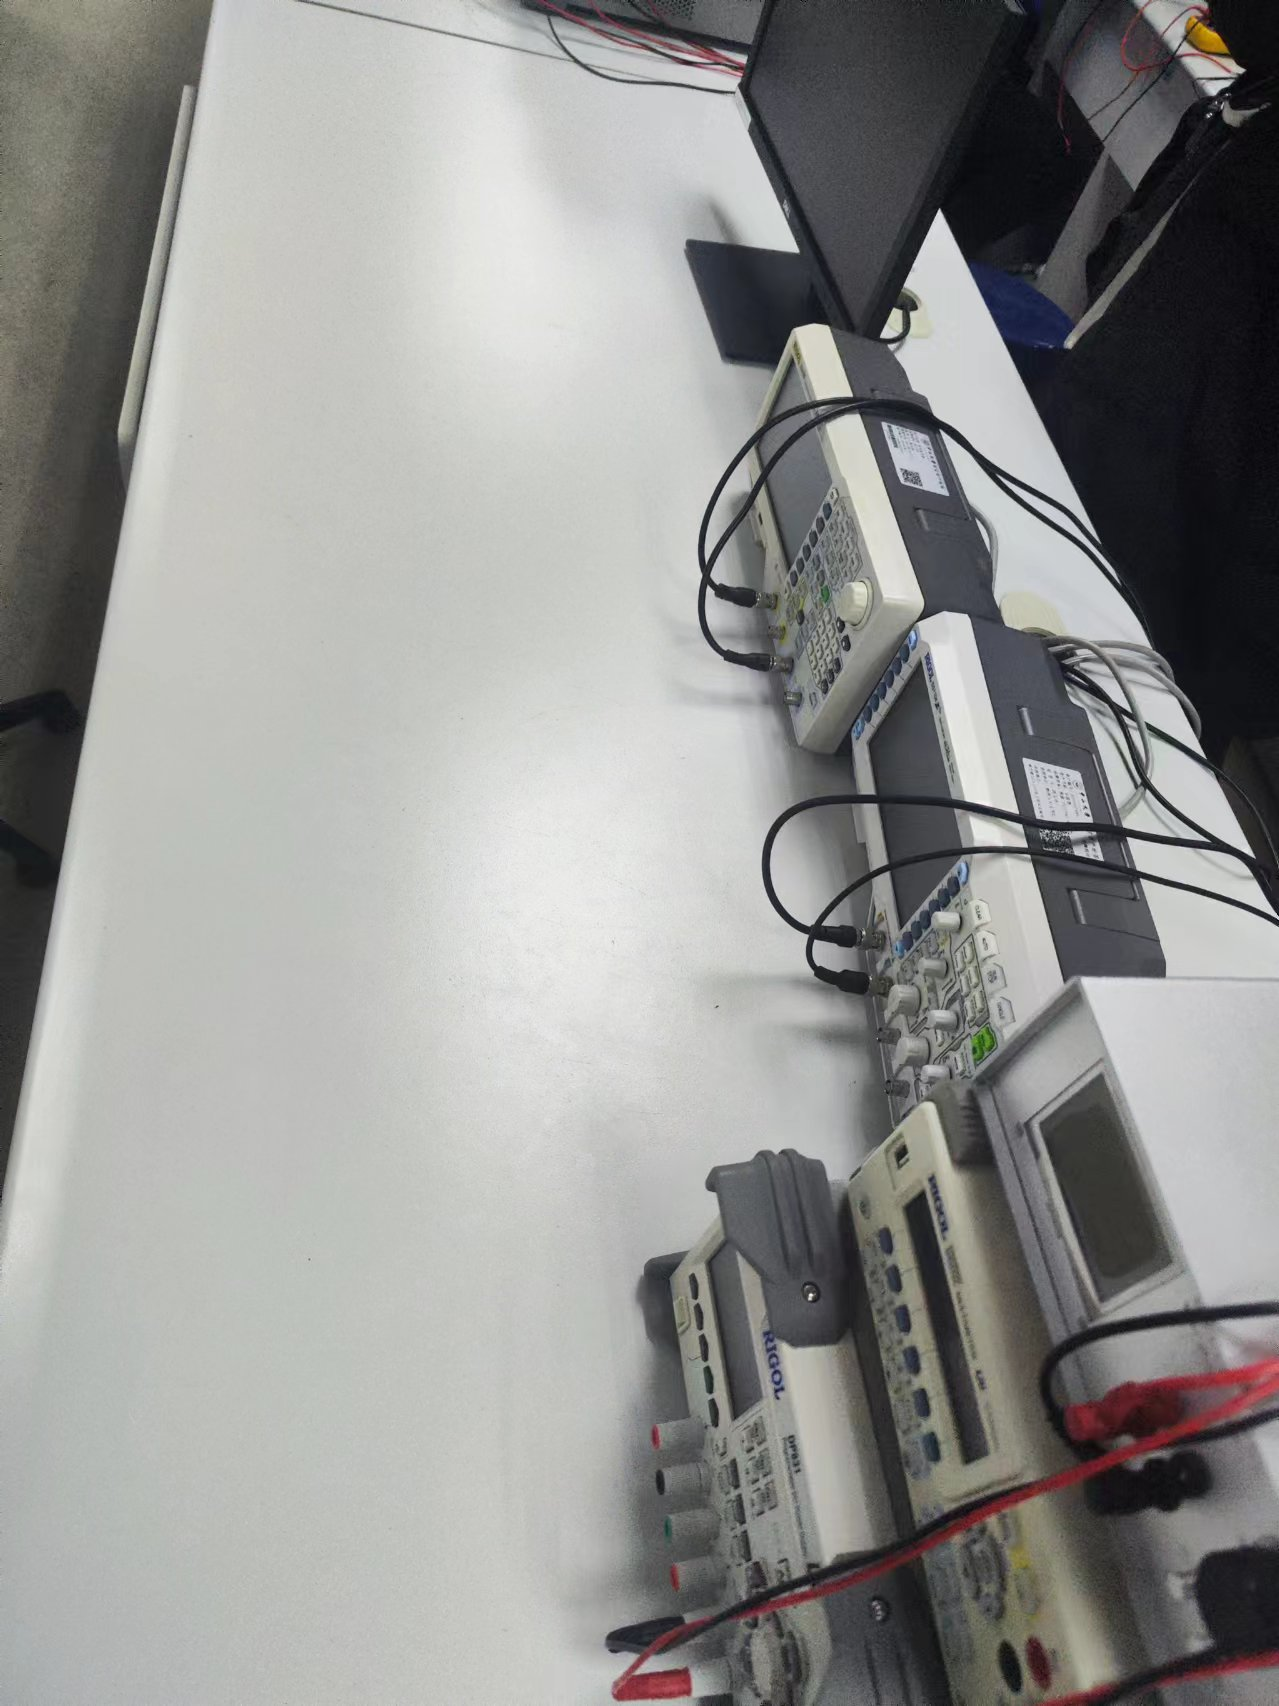
\includegraphics[width=0.4\linewidth]{桌面.jpg}
		\caption{桌面整理}
		\label{}
	\end{figure}
	

	
	
	
	
\end{document}